% Options for packages loaded elsewhere
\PassOptionsToPackage{unicode}{hyperref}
\PassOptionsToPackage{hyphens}{url}
\documentclass[
  ignorenonframetext,
  aspectratio=169,
]{beamer}
\newif\ifbibliography
\usepackage{pgfpages}
\setbeamertemplate{caption}[numbered]
\setbeamertemplate{caption label separator}{: }
\setbeamercolor{caption name}{fg=normal text.fg}
\beamertemplatenavigationsymbolsempty
% remove section numbering
\setbeamertemplate{part page}{
  \centering
  \begin{beamercolorbox}[sep=16pt,center]{part title}
    \usebeamerfont{part title}\insertpart\par
  \end{beamercolorbox}
}
\setbeamertemplate{section page}{
  \centering
  \begin{beamercolorbox}[sep=12pt,center]{section title}
    \usebeamerfont{section title}\insertsection\par
  \end{beamercolorbox}
}
\setbeamertemplate{subsection page}{
  \centering
  \begin{beamercolorbox}[sep=8pt,center]{subsection title}
    \usebeamerfont{subsection title}\insertsubsection\par
  \end{beamercolorbox}
}
% Prevent slide breaks in the middle of a paragraph
\widowpenalties 1 10000
\raggedbottom
\AtBeginPart{
  \frame{\partpage}
}
\AtBeginSection{
  \ifbibliography
  \else
    \frame{\sectionpage}
  \fi
}
\AtBeginSubsection{
  \frame{\subsectionpage}
}
\usepackage{iftex}
\ifPDFTeX
  \usepackage[T1]{fontenc}
  \usepackage[utf8]{inputenc}
  \usepackage{textcomp} % provide euro and other symbols
\else % if luatex or xetex
  \usepackage{unicode-math} % this also loads fontspec
  \defaultfontfeatures{Scale=MatchLowercase}
  \defaultfontfeatures[\rmfamily]{Ligatures=TeX,Scale=1}
\fi
\usepackage{lmodern}
\ifPDFTeX\else
  % xetex/luatex font selection
\fi
% Use upquote if available, for straight quotes in verbatim environments
\IfFileExists{upquote.sty}{\usepackage{upquote}}{}
\IfFileExists{microtype.sty}{% use microtype if available
  \usepackage[]{microtype}
  \UseMicrotypeSet[protrusion]{basicmath} % disable protrusion for tt fonts
}{}
\makeatletter
\@ifundefined{KOMAClassName}{% if non-KOMA class
  \IfFileExists{parskip.sty}{%
    \usepackage{parskip}
  }{% else
    \setlength{\parindent}{0pt}
    \setlength{\parskip}{6pt plus 2pt minus 1pt}}
}{% if KOMA class
  \KOMAoptions{parskip=half}}
\makeatother
\usepackage{longtable,booktabs,array}
\usepackage{caption}
\captionsetup[table]{skip=6pt}
\newcounter{none} % for unnumbered tables
\usepackage{calc} % for calculating minipage widths
\usepackage{caption}
% Make caption package work with longtable
\makeatletter
\def\fnum@table{\tablename~\thetable}
\makeatother
\usepackage{graphicx}
\makeatletter
\newsavebox\pandoc@box
\newcommand*\pandocbounded[1]{% scales image to fit in text height/width
  \sbox\pandoc@box{#1}%
  \Gscale@div\@tempa{\textheight}{\dimexpr\ht\pandoc@box+\dp\pandoc@box\relax}%
  \Gscale@div\@tempb{\linewidth}{\wd\pandoc@box}%
  \ifdim\@tempb\p@<\@tempa\p@\let\@tempa\@tempb\fi% select the smaller of both
  \ifdim\@tempa\p@<\p@\scalebox{\@tempa}{\usebox\pandoc@box}%
  \else\usebox{\pandoc@box}%
  \fi%
}
% Set default figure placement to htbp
\def\fps@figure{htbp}
\makeatother
\setlength{\emergencystretch}{3em} % prevent overfull lines
\providecommand{\tightlist}{%
  \setlength{\itemsep}{0pt}\setlength{\parskip}{0pt}}
% Auto-generated by infrastructure/rendering/_pdf_latex_helpers.py::extract_math_font_preamble.
% Minimal header passed to Pandoc via -H so Beamer slides pick up the same math font
% as the combined-PDF path. Adjust the manuscript's preamble.md to change the font globally.
\usepackage{unicode-math}
\setmathfont{latinmodern-math.otf}

% Manuscript macro/package fallbacks (newcommand -> providecommand).
% Core mathematics
\usepackage{amsmath}
\usepackage{amssymb}
% Document layout
% Tables
\usepackage{booktabs}
% Caption styling (booktabs already loaded above). Small caption font with a
% bold label ("Figure 1", "Table 2") gives the math/figure-heavy layout a
% consistent, journal-like caption rhythm without fighting pandoc-crossref —
% pandoc emits standard \caption{}, and caption/captionsetup only restyle it.
% ── Theorem environments ─────────────────────────────────────────────────
% amsthm is loaded above. The FedGVI<->Friston bridge is stated as a small
% number of theorems/definitions/lemmas/propositions/corollaries; sharing one
% counter (definition/lemma/proposition/corollary all step the `theorem`
% counter) gives a single monotone numbering 1, 2, 3, ... across all kinds, so
% authors can reference them as Theorem 1, Definition 2, Corollary 3 without a
% per-kind counter drifting out of order. Plain style for theorem-like results,
% definition style (upright body) for definitions.
% (algorithm2e intentionally not loaded: this manuscript states results as
% numbered amsthm Theorems/Definitions, not algorithm2e pseudocode.)
% Code listings
\usepackage{listings}
% Typography and formatting
% (siunitx intentionally not loaded: no \SI/\num units appear in this manuscript.)
% Cross-references and citations
% (cleveref and titlesec intentionally not loaded: unavailable in this TeX tree
% and not required. Cross-references resolve through pandoc-crossref's own
% \ref-style names — no \cref appears — and section heading styling falls back
% to the pandoc/LaTeX defaults.)
% ── TeX Live Basic-compatible mono font for code listings ────────────
% Latin Modern Mono is bundled with TeX Live Basic and keeps the manuscript
% renderable on minimal TeX installations. Mathematical Unicode coverage is
% provided separately by Latin Modern Math below, so the code font does not
% need a private JuliaMono installation.
%
% Use the TeX font filename rather than the system-family name: the minimal
% TeX Live fontconfig database may not register the OpenType family even though
% kpsewhich can resolve the bundled files.
% Math font for unicode-math: Latin Modern Math (TeX Live) has full BMP
% coverage including U+2223 (\mid), U+226A/226B (\ll/\gg), and the Greek/
% blackboard letters used in equations. Without an explicit \setmathfont,
% unicode-math falls back to lmroman text font which lacks several glyphs
% and emits "Missing character" warnings on every \mid in math mode.

% Slide layout defaults for warning-clean scientific decks.
\usepackage{etoolbox}
\IfFileExists{xurl.sty}{\usepackage{xurl}}{}
\IfFileExists{seqsplit.sty}{\usepackage{seqsplit}}{\newcommand{\seqsplit}[1]{#1}}
\protected\def\breakseq#1{\seqsplit{#1}}
\protected\def\breaktt#1{\begingroup\ttfamily\seqsplit{#1}\endgroup}
\setlength{\emergencystretch}{6em}
\tolerance=5000
\hbadness=10000
\hfuzz=1pt
\setlength{\tabcolsep}{2pt}
\AtBeginEnvironment{longtable}{\tiny\renewcommand{\arraystretch}{0.86}\setlength{\tabcolsep}{1pt}}
\AtBeginEnvironment{tabular}{\tiny\renewcommand{\arraystretch}{0.86}\setlength{\tabcolsep}{1pt}}
\AtBeginEnvironment{equation}{\tiny}
\AtBeginEnvironment{equation*}{\tiny}
\AtBeginEnvironment{align}{\tiny}
\AtBeginEnvironment{align*}{\tiny}
\AtBeginEnvironment{itemize}{\footnotesize}
\AtBeginEnvironment{enumerate}{\footnotesize}
\AtBeginEnvironment{description}{\footnotesize}
\setbeamerfont{caption}{size=\tiny}
\setbeamerfont{caption name}{size=\tiny}
\setbeamerfont{normal text}{size=\small}
\setbeamerfont{frametitle}{size=\small}
\setbeamerfont{section title}{size=\footnotesize}
\setbeamerfont{subsection title}{size=\footnotesize}
\setbeamertemplate{section page}{%
  \centering
  \begin{beamercolorbox}[sep=12pt,center,wd=\paperwidth]{section title}
    \parbox{0.86\paperwidth}{\centering\usebeamerfont{section title}\insertsection\par}
  \end{beamercolorbox}
}
\setbeamertemplate{subsection page}{%
  \centering
  \begin{beamercolorbox}[sep=8pt,center,wd=\paperwidth]{subsection title}
    \parbox{0.86\paperwidth}{\centering\usebeamerfont{subsection title}\insertsubsection\par}
  \end{beamercolorbox}
}
\setlength{\abovecaptionskip}{2pt}
\setlength{\belowcaptionskip}{0pt}

% Natbib and cross-reference fallbacks — slides don't load natbib
% or cleveref, but combined-PDF manuscript prose may emit these
% commands. The fallback renders citations as a bracketed key list
% and cross-references as detokenized labels so slides don't fail on
% undefined control sequences or raw underscores. \providecommand is
% a no-op if packages load later.
\providecommand{\citep}[1]{[#1]}
\providecommand{\citet}[1]{#1}
\providecommand{\citealp}[1]{#1}
\providecommand{\citeauthor}[1]{#1}
\providecommand{\citeyear}[1]{#1}
\providecommand{\cref}[1]{\texttt{\detokenize{#1}}}
\providecommand{\Cref}[1]{\texttt{\detokenize{#1}}}
\providecommand{\crefrange}[2]{\texttt{\detokenize{#1}}--\texttt{\detokenize{#2}}}
\providecommand{\Crefrange}[2]{\texttt{\detokenize{#1}}--\texttt{\detokenize{#2}}}
\providecommand{\paragraph}[1]{\textbf{#1}\ }

% Opt-in accessible presentation profile.
\setbeamerfont{normal text}{size*={20pt}{24pt}}
\setbeamerfont{frametitle}{size*={28pt}{32pt}}
\setbeamerfont{section title}{size*={28pt}{32pt}}
\setbeamerfont{subsection title}{size*={28pt}{32pt}}
\setbeamerfont{caption}{size*={16pt}{19pt}}
\setbeamerfont{caption name}{size*={16pt}{19pt}}
\setbeamerfont{itemize/enumerate body}{size*={20pt}{24pt}}
\setbeamerfont{itemize/enumerate subbody}{size*={20pt}{24pt}}
\setbeamerfont{itemize/enumerate subsubbody}{size*={20pt}{24pt}}
\setbeamerfont{itemize item}{size*={20pt}{24pt}}
\setbeamerfont{itemize subitem}{size*={20pt}{24pt}}
\setbeamerfont{itemize subsubitem}{size*={20pt}{24pt}}
\setbeamerfont{description body}{size*={20pt}{24pt}}
\setbeamerfont{description item}{size*={20pt}{24pt}}
\setbeamerfont{quote}{size*={20pt}{24pt}}
\setbeamerfont{quotation}{size*={20pt}{24pt}}
\AtBeginEnvironment{longtable}{\fontsize{20pt}{24pt}\selectfont}
\AtBeginEnvironment{tabular}{\fontsize{20pt}{24pt}\selectfont}
\AtBeginEnvironment{equation}{\fontsize{20pt}{24pt}\selectfont}
\AtBeginEnvironment{equation*}{\fontsize{20pt}{24pt}\selectfont}
\AtBeginEnvironment{align}{\fontsize{20pt}{24pt}\selectfont}
\AtBeginEnvironment{align*}{\fontsize{20pt}{24pt}\selectfont}
\AtBeginEnvironment{itemize}{\fontsize{20pt}{24pt}\selectfont}
\AtBeginEnvironment{enumerate}{\fontsize{20pt}{24pt}\selectfont}
\AtBeginEnvironment{description}{\fontsize{20pt}{24pt}\selectfont}
\AtBeginDocument{\usebeamerfont{normal text}}
\newlength{\AFSlideTableWidth}
% The fixed footer reservation is calibrated with the semantic seven-line regular-body budget.
\setbeamertemplate{footline}{%
  \leavevmode\vbox{%
    \hbox{%
      \begin{beamercolorbox}[wd=\paperwidth,ht=16pt,dp=3pt,center]{author in head/foot}%
        \fontsize{16pt}{19pt}\selectfont Untagged PDF derivative \textbar\ \href{../web/index.html}{HTML reader}%
      \end{beamercolorbox}%
    }%
    \vskip6pt%
  }%
}
% Accessible footer reserved height: 25pt.

\newtheorem{proposition}{Proposition}
\newtheorem{hypothesis}{Hypothesis}
\newtheorem{remark}[theorem]{Remark}
\newtheorem{axiom}{Axiom}
\newtheorem{property}{Property}
\usepackage{bookmark}
\IfFileExists{xurl.sty}{\usepackage{xurl}}{} % add URL line breaks if available
\urlstyle{same}
% fallback for those not using the hyperref driver hyperxmp:
\makeatletter
\@ifundefined{xmpquote}{\newcommand{\xmpquote}[1]{#1}}{}
\makeatother
\hypersetup{
  hidelinks,
  pdfcreator={LaTeX via pandoc}}

\author{\texorpdfstring{}{}}
\date{}

\begin{document}

\section{Introduction: from belief sharing to robust generalized
Bayes}\label{sec:introduction}

\begin{frame}{Introduction: from belief sharing to robust generalized
Bayes}
A colony of active-inference agents that shares beliefs inherits both
the power and the fragility of the pool it uses: the same multiplication
of reports that sharpens an honest consensus lets a single confident,
wrong member capture it.
\end{frame}

\begin{frame}{Introduction (part 2)}
Two research communities each hold part of the remedy but do not, on
their own, close the gap.
\end{frame}

\begin{frame}{Introduction (part 3)}
The active-inference community gives agents generative models, action
selection, and colony-level belief sharing. The robust- and
federated-Bayes community gives generalized objectives and aggregation
methods for inference under misspecification or contamination.
\end{frame}

\begin{frame}{Introduction (part 4)}
The cited literatures do not, however, provide a single tested treatment
of robust categorical belief fusion for active-inference agents. This
introduction states the problem and its evidence boundary;
sec.~3 scopes the reviewed gap,
\end{frame}

\begin{frame}{Introduction (part 5)}
and sec.~4 lists the contributions together with
what each result does not establish.
\end{frame}

\begin{frame}{Active inference supplies generative agents and shared
beliefs}
\protect\phantomsection\label{sec:intro-active-inference}
Active inference casts perception, learning, and action as the
minimization of variational free energy under a generative model,
\end{frame}

\begin{frame}{Active inference supplies\ldots{} (part 2)}
a program that grew out of the free-energy principle (Friston 2010) and
its process-theory implementation (Friston et al. 2017).
\end{frame}

\begin{frame}{Active inference supplies\ldots{} (part 3)}
In the discrete state-space setting the formalism is now standardized.
An agent carries the categorical tensors \(A\) (likelihood), \(B\)
(transitions), \(C\) (preferences), and \(D_0\) (initial priors), and
infers hidden states by minimizing variational free energy. It selects
actions by minimizing \emph{expected} free energy ---
\end{frame}

\begin{frame}{Active inference supplies\ldots{} (part 4)}
the sum of a risk term and an ambiguity term that together trade off
goal-seeking against uncertainty-resolving behavior (Da Costa et al.
2020).
\end{frame}

\begin{frame}{Active inference supplies\ldots{} (part 5)}
This synthesis is the substrate we build on. Mature toolboxes make it
executable at scale: pymdp provides discrete-state active inference in
Python (Heins et al. 2022), and RxInfer delivers reactive message
passing for exact Bayesian inference (Bagaev et al. 2023).
\end{frame}

\begin{frame}{Active inference supplies\ldots{} (part 6)}
The community has also moved from single agents to \emph{collectives}.
Surprise-minimizing ensembles reproduce collective animal behavior such
as schooling and flocking (Heins et al. 2024); epistemic communities
form when agents share a generative model and exchange evidence
(Albarracin et al. 2022);
\end{frame}

\begin{frame}{Active inference supplies\ldots{} (part 7)}
and collective intelligence has been framed directly in active-inference
terms (Kaufmann et al. 2021).
\end{frame}

\begin{frame}{Active inference supplies\ldots{} (part 8)}
The narrow bridge studied here starts from posterior broadcasts over one
shared categorical factor --- a predator's location, say --- and forms a
project log-linear pool (eq.~9). Under the
explicit finite-shared-support, posterior-log-potential,
\end{frame}

\begin{frame}{Active inference supplies\ldots{} (part 9)}
and fixed-weight assumptions of sec.~5.8, that
weighted geometric pool is a specialization of Friston et al.'s Eq. 7
message-combination term (Friston et al. 2024).
\end{frame}

\begin{frame}{Active inference supplies\ldots{} (part 10)}
It is not a reconstruction of the source message construction,
scheduling, cavity policy, generative factors, or complete protocol.
That representation connects the qualified categorical bridge to the
classical logarithmic-pooling literature (Genest and Zidek 1986; Genest
et al. 1986),
\end{frame}

\begin{frame}{Active inference supplies\ldots{} (part 11)}
to modern Bayesian treatments of log-pool weights (Carvalho et al.
2023), to product-of-experts geometry in machine learning (Hinton 2002),
and to distributed Bayesian estimators (Tresp 2000). In the reproduced
baseline,
\end{frame}

\begin{frame}{Active inference supplies\ldots{} (part 12)}
communication lowers mean free energy relative to the matched
incommunicado condition (sec.~7.2).
\end{frame}

\begin{frame}{Active inference supplies\ldots{} (part 13)}
Friston et al. (2024) crystallized the colony mechanism into three
worked simulations --- communicating-colony free-energy convergence,
Dirichlet language acquisition, and Bayesian model reduction structure
emergence ---
\end{frame}

\begin{frame}{Active inference supplies\ldots{} (part 14)}
whose mechanisms motivate three reduced categorical analogues in this
repository (sec.~7.1). They are not numerical or
exact protocol replications; a source-parity reconstruction remains
future work before evaluating source-level equivalence.
\end{frame}

\begin{frame}{Active inference supplies\ldots{} (part 15)}
Alongside fusion, the community has tools for growing the model itself:
active inference connects naturally to Bayesian optimal experimental
design and model selection (Smith et al. 2022),
\end{frame}

\begin{frame}{Active inference supplies\ldots{} (part 16)}
and post-hoc Bayesian model reduction prunes redundant structure by
comparing free-energy bounds (Friston and Penny 2011) --- the algebra
used by our configured BMR sign control
(sec.~7.4).
\end{frame}

\begin{frame}{Active inference supplies\ldots{} (part 17)}
The reviewed active-inference belief-sharing work does not
systematically characterize fusion under explicit contamination or
intentionally wrong belief broadcasts.
\end{frame}

\begin{frame}{Active inference supplies\ldots{} (part 18)}
The log-linear pool assumes reports are compatible with the shared
generative model, while the opinion-pooling literature makes the
assumptions about independence, weights, and external Bayesian coherence
explicit (Genest and Zidek 1986; Genest et al. 1986). Fully Bayesian
aggregation sharpens the point:
\end{frame}

\begin{frame}{Active inference supplies\ldots{} (part 19)}
geometric pooling is normatively compelling under dynamic-Bayesian
rationality assumptions, not an assumption-free robustness procedure
(Dietrich 2021).
\end{frame}

\begin{frame}{Active inference supplies\ldots{} (part 20)}
The same product geometry can be brittle: if a report assigns zero or
near-zero mass to the true state, the product can assign near-zero mass
there too. That is the failure mode tested here, not a claim that every
federation or every product pool behaves identically.
\end{frame}

\begin{frame}{Robust and federated Bayes supplies bounded-influence
updating}
\protect\phantomsection\label{sec:intro-robust-bayes}
A separate literature studies bounded-influence updating outside active
inference. \textbf{Federated learning} aggregates models trained on
decentralized data without pooling the data itself,
\end{frame}

\begin{frame}{Robust and federated Bayes\ldots{} (part 2)}
the canonical algorithm being FedAvg (McMahan et al. 2017).
\end{frame}

\begin{frame}{Robust and federated Bayes\ldots{} (part 3)}
Cast probabilistically, federated and continual learning unify under
\textbf{partitioned variational inference}, in which each client owns a
factor of a global approximate posterior and the server combines factors
in natural-parameter space (Bui et al. 2018; Ashman et al. 2022).
\end{frame}

\begin{frame}{Robust and federated Bayes\ldots{} (part 4)}
This is a closely related factor algebra expressed in a different
vocabulary; the implementation tests the correspondence in the
categorical recovery limit rather than assuming that the two settings
are interchangeable.
\end{frame}

\begin{frame}{Robust and federated Bayes\ldots{} (part 5)}
The robustness this paper needs comes from \textbf{generalized Bayesian
inference}, which replaces the likelihood with a \emph{loss} and the KL
regularizer with a \emph{general divergence},
\end{frame}

\begin{frame}{Robust and federated Bayes\ldots{} (part 6)}
so that the posterior minimizes a generalized objective rather than
applying Bayes' rule literally (Bissiri et al. 2016; Jewson et al. 2018;
Knoblauch et al. 2022).
\end{frame}

\begin{frame}{Robust and federated Bayes\ldots{} (part 7)}
This includes Gibbs-posterior updates (Jiang and Tanner 2008), coarsened
or tempered posteriors that condition on neighborhoods rather than exact
data (Miller and Dunson 2018),
\end{frame}

\begin{frame}{Robust and federated Bayes\ldots{} (part 8)}
and learning-rate/temperature choices designed for safe updating under
misspecification (Grünwald 2012; Kleijn and Vaart 2012). Choosing a loss
or divergence with a bounded-influence property --- for example,
\end{frame}

\begin{frame}{Robust and federated Bayes\ldots{} (part 9)}
the density-power \(\beta\)-loss (Basu et al. 1998; Fujisawa and Eguchi
2008; Ghosh and Basu 2015) or generalized cross-entropy (Zhang and
Sabuncu 2018) --- can cap the influence of a contaminated observation
under the corresponding assumptions.
\end{frame}

\begin{frame}{Robust and federated Bayes\ldots{} (part 10)}
\textbf{FedGVI} (Mildner et al. 2025) federates this idea: each client
runs a robust generalized-Bayes update against a \emph{cavity} (the
global posterior with the client's own factor removed), and the server
aggregates the refreshed factors under a chosen server divergence.
\end{frame}

\begin{frame}{Robust and federated Bayes\ldots{} (part 11)}
The result is federated inference with divergence- and loss-specific
robustness guarantees, demonstrated on Bayesian neural networks under
label contamination.
\end{frame}

\begin{frame}{Robust and federated Bayes\ldots{} (part 12)}
Crucially, standard Bayes is a \emph{corner} of this generalized family
--- the case where the loss is the negative log-likelihood and the
divergence is KL. Friston et al.~do not claim FedGVI, generalized Bayes,
\(\beta\)-divergence, or robustness; this manuscript supplies the
recasting.
\end{frame}

\begin{frame}{Robust and federated Bayes\ldots{} (part 13)}
Robust generalized Bayes therefore does not replace exact-Bayes belief
fusion; it contains the standard pool as a tested zero-robustness
recovery limit. That containment is the hinge this paper tests,
\end{frame}

\begin{frame}{Robust and federated Bayes\ldots{} (part 14)}
and the recovery limits are stated formally as numbered results in
sec.~6 and the central identity in
sec.~5.8.
\end{frame}

\begin{frame}{Robust and federated Bayes\ldots{} (part 15)}
The historical framing is deliberately modest. The manuscript uses early
probability, inverse-probability, utility, and collective-judgment
sources as a conceptual genealogy for belief, evidence, expectation,
\end{frame}

\begin{frame}{Robust and federated Bayes\ldots{} (part 16)}
and aggregation (Pascal and Fermat 1654; Huygens 1657; Bernoulli 1713;
Moivre 1718; Bayes 1763; Laplace 1774; Bernoulli 1738; Condorcet 1785).
These sources do not anticipate KL divergence, product-of-experts
learning, variational Bayes, or federated optimization;
\end{frame}

\begin{frame}{Robust and federated Bayes\ldots{} (part 17)}
the modern correspondence to FedGVI is the formal construction proved
and tested here.
\end{frame}

\begin{frame}{Robust and federated Bayes\ldots{} (part 18)}
Beyond this core, we evaluate a tempered objective family, a
deterministic MLP aggregation transfer, and disjoint-field-of-view
communication. These are boundary tests: the first probes the
accuracy/weight-control trade-off, the second tests API portability in
one additional model class,
\end{frame}

\begin{frame}{Robust and federated Bayes\ldots{} (part 19)}
and the third separates a binary-complement null result from a
larger-state-space case where communication materially improves
consensus.
\end{frame}

\begin{frame}{Questions, design, and evidence boundary}
\protect\phantomsection\label{sec:intro-questions}
The paper answers four scoped questions. First, does turning robustness
off recover the standard log-linear pool and closed-form Bayes update?
Second, under the declared confident-wrong broadcast mechanism,
\end{frame}

\begin{frame}{Questions, design, and\ldots{} (part 2)}
how does the server heuristic change consensus accuracy across
contamination rates? Third, what does the objective-backed variational
server rule guarantee, and what accuracy does it trade away? Fourth,
\end{frame}

\begin{frame}{Questions, design, and\ldots{} (part 3)}
how do communication, hierarchy, sensitivity, and parameter recovery
behave in the accompanying categorical extensions?
\end{frame}

\begin{frame}{Questions, design, and\ldots{} (part 4)}
The first question is answered algebraically and by machine-precision
checks; the others are conditional simulation results. The independent
unit, resampling scheme, and fixed hidden-state/attack-target estimand
are specified in sec.~5.22 and
sec.~5.27.
\end{frame}

\begin{frame}{How to read the visual architecture}
\protect\phantomsection\label{sec:intro-visual-map}
The manuscript uses two complementary visual layers. The formal
schematics adapt the generative-model and posterior-sharing perspective
of Friston et al. (2024) to the categorical implementation:
fig.~4 shows the private sensory report
and \(A/B/C/D\) substrate,
\end{frame}

\begin{frame}{How to read the visual\ldots{} (part 2)}
fig.~3 shows how three local posterior messages
become server inputs, and fig.~5 shows the
hidden-state, agent, and active-control context. These diagrams are
explanatory maps, not additional empirical observations.
\end{frame}

\begin{frame}{How to read the visual\ldots{} (part 3)}
The data-bearing figures then report the executed recovery checks,
conditional contamination sweep, and objective/descent diagnostics;
their captions identify the relevant uncertainty and resampling unit.
\end{frame}

\begin{frame}{How to read the visual\ldots{} (part 4)}
The graphical abstract in fig.~1 compresses
the same logic into a recovery anchor, a federation pathway, and three
explicitly non-transferable robustness axes.
\end{frame}

\begin{frame}{How to read the visual\ldots{} (part 5)}
fig.~2 illustrates one configured
failure-and-repair case: a partially contaminated colony broadcasts
beliefs (Panel A), the equal-weight log-linear pool is pulled toward the
attack target (Panel B), and the server-side heuristic reweights the
broadcasts (Panel C). It is a deterministic schematic,
\end{frame}

\begin{frame}{How to read the visual\ldots{} (part 6)}
not a universal robustness claim; the three axes and their distinct
guarantees are defined in sec.~3 and
sec.~3.3.
\end{frame}

\begin{frame}{How to read the visual\ldots{} (part 7)}
\begin{figure}
\centering
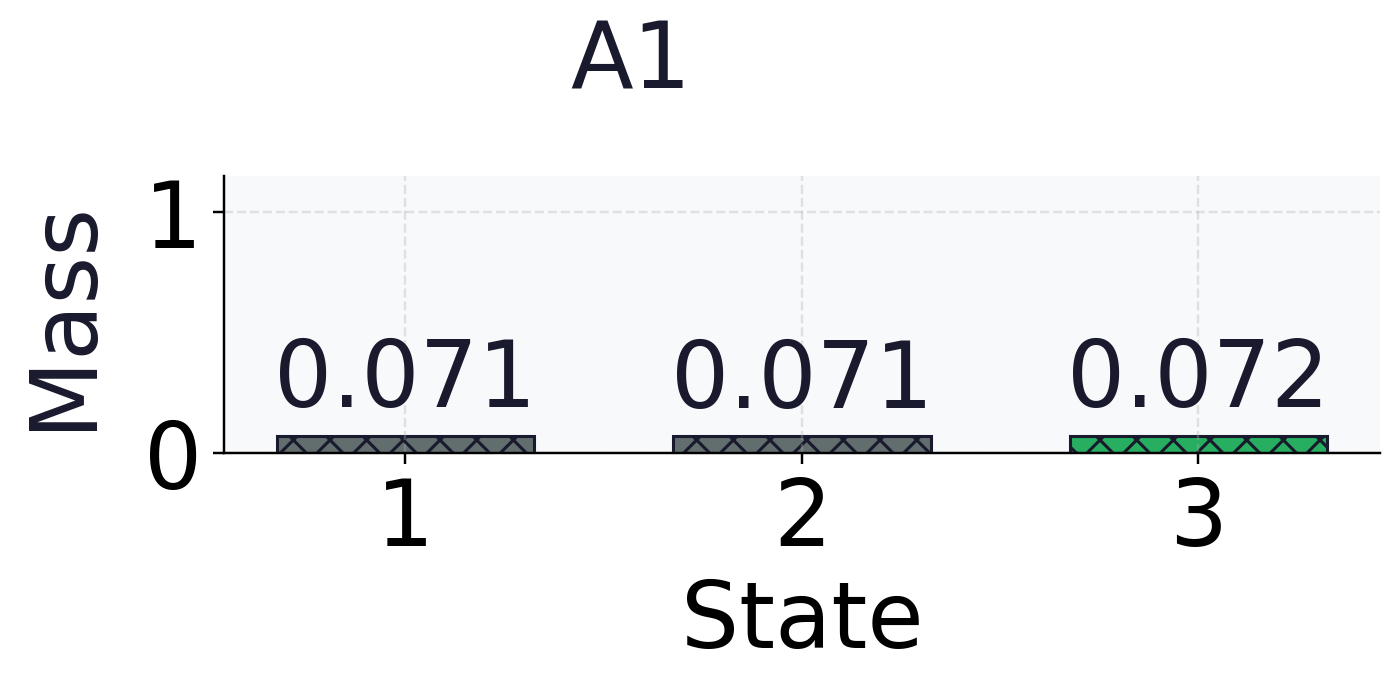
\includegraphics[keepaspectratio,width=0.98\linewidth,height=0.8\textheight,alt={A1: source-derived posterior masses for states 1 to 3, common 0--1 probability scale; arrow marks this row\textquotesingle s argmax when present.}]{../figures/system_overview.slide-row-1-states-1-3.png}
\refstepcounter{figure}\label{fig:system-overview-slide-panel-1}
\end{figure}
\end{frame}

\begin{frame}{How to read the visual\ldots{} (part 8)}
\begin{figure}
\centering
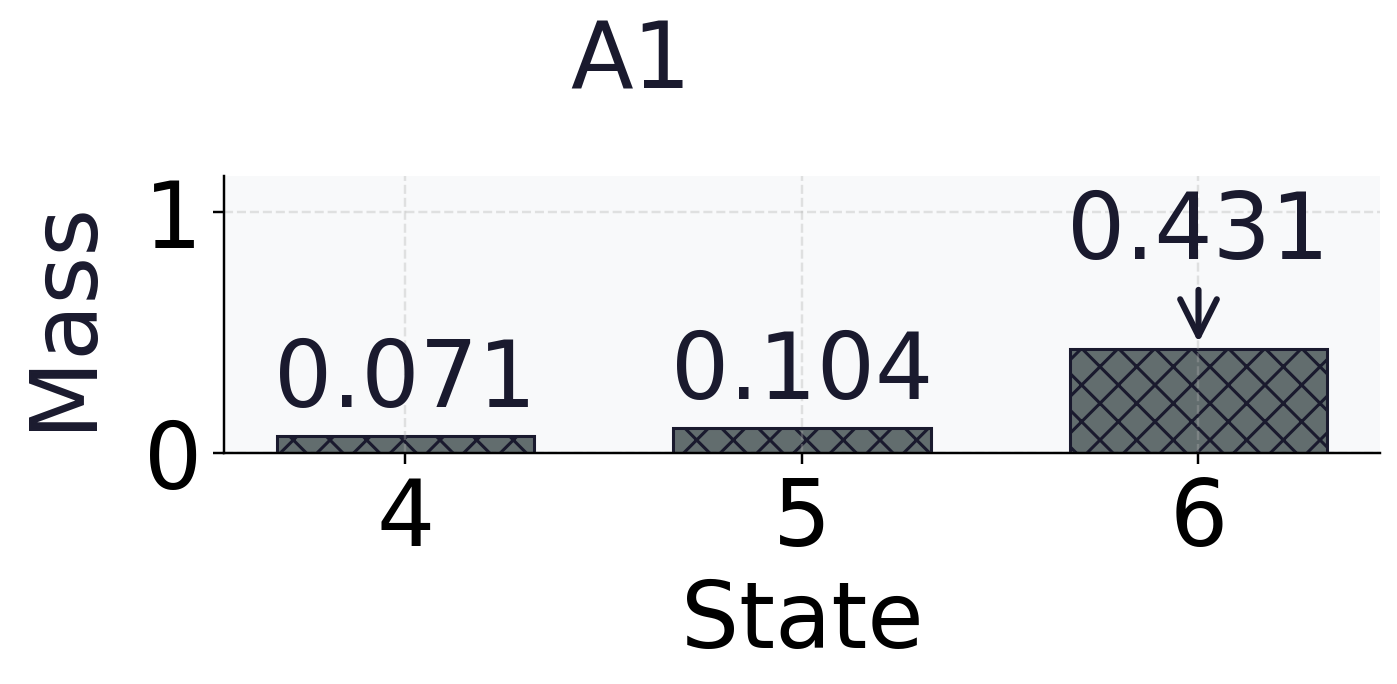
\includegraphics[keepaspectratio,width=0.98\linewidth,height=0.8\textheight,alt={A1: source-derived posterior masses for states 4 to 6, common 0--1 probability scale; arrow marks this row\textquotesingle s argmax when present.}]{../figures/system_overview.slide-row-1-states-4-6.png}
\refstepcounter{figure}\label{fig:system-overview-slide-panel-2}
\end{figure}
\end{frame}

\begin{frame}{How to read the visual\ldots{} (part 9)}
\begin{figure}
\centering
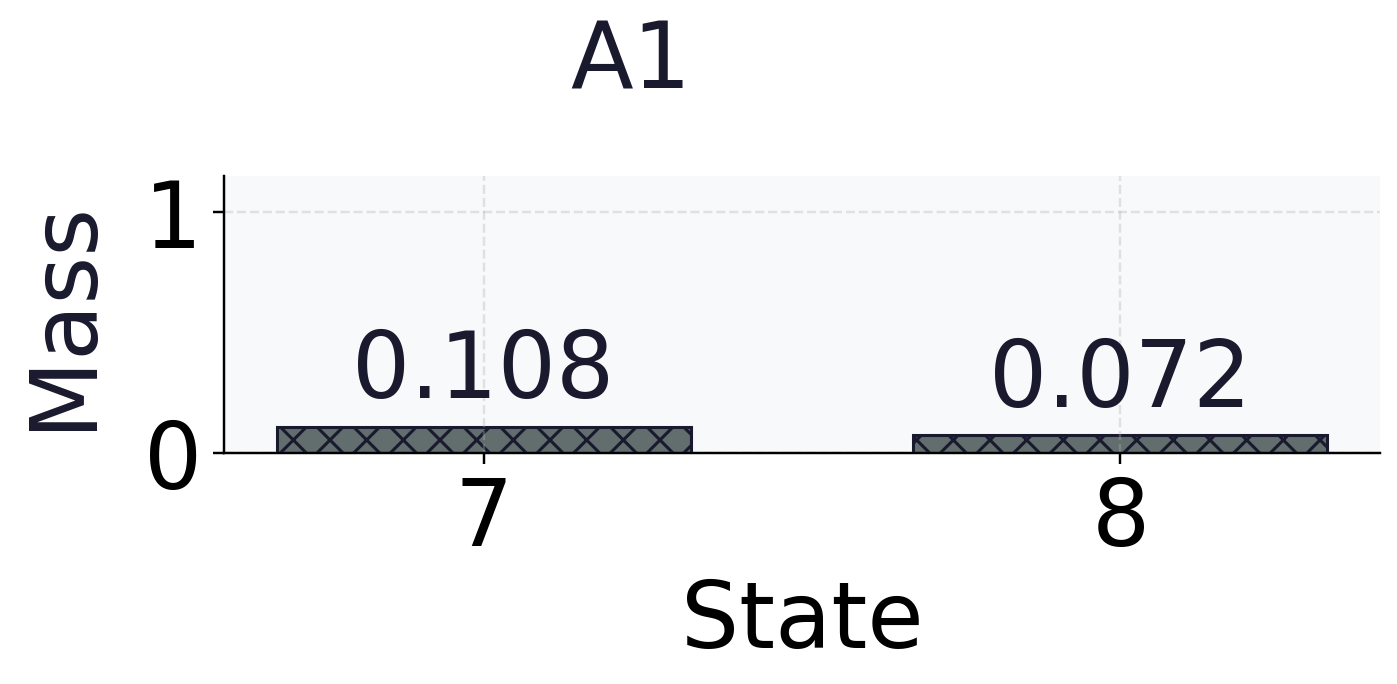
\includegraphics[keepaspectratio,width=0.98\linewidth,height=0.8\textheight,alt={A1: source-derived posterior masses for states 7 to 8, common 0--1 probability scale; arrow marks this row\textquotesingle s argmax when present.}]{../figures/system_overview.slide-row-1-states-7-8.png}
\refstepcounter{figure}\label{fig:system-overview-slide-panel-3}
\end{figure}
\end{frame}

\begin{frame}{How to read the visual\ldots{} (part 10)}
\begin{figure}
\centering
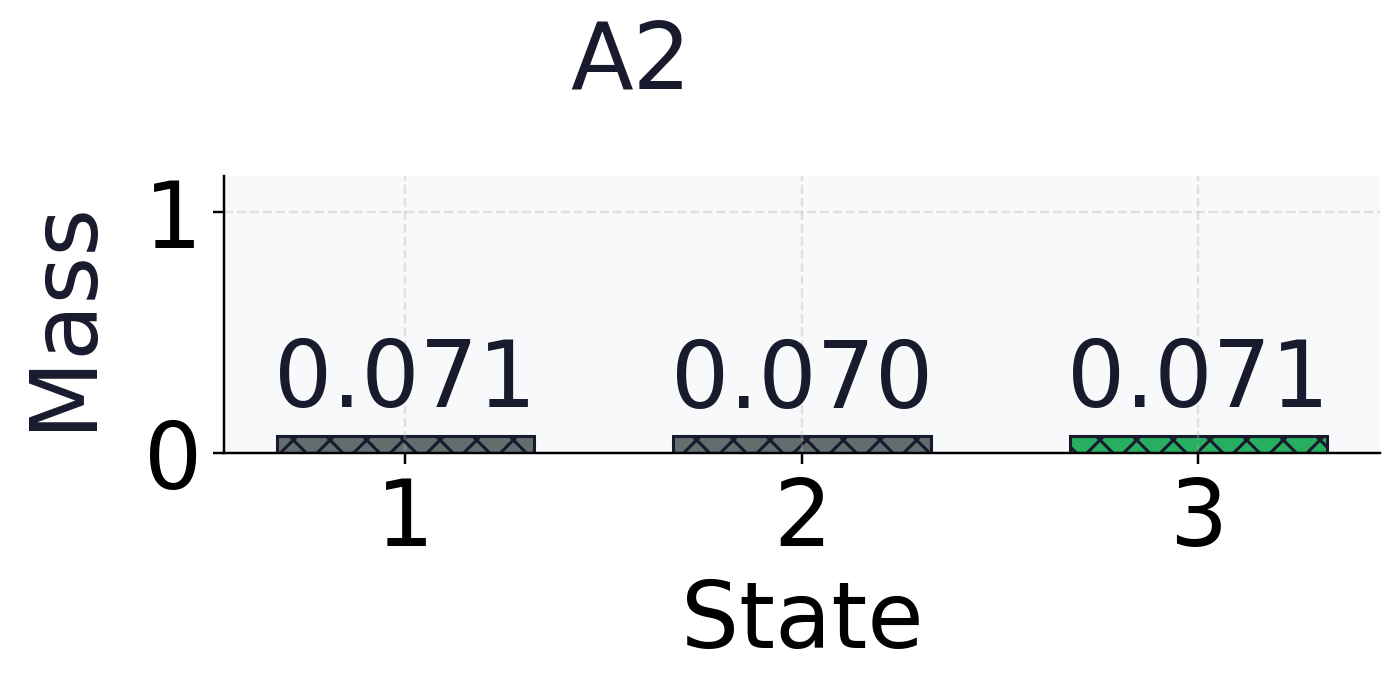
\includegraphics[keepaspectratio,width=0.98\linewidth,height=0.8\textheight,alt={A2: source-derived posterior masses for states 1 to 3, common 0--1 probability scale; arrow marks this row\textquotesingle s argmax when present.}]{../figures/system_overview.slide-row-2-states-1-3.png}
\refstepcounter{figure}\label{fig:system-overview-slide-panel-4}
\end{figure}
\end{frame}

\begin{frame}{How to read the visual\ldots{} (part 11)}
\begin{figure}
\centering
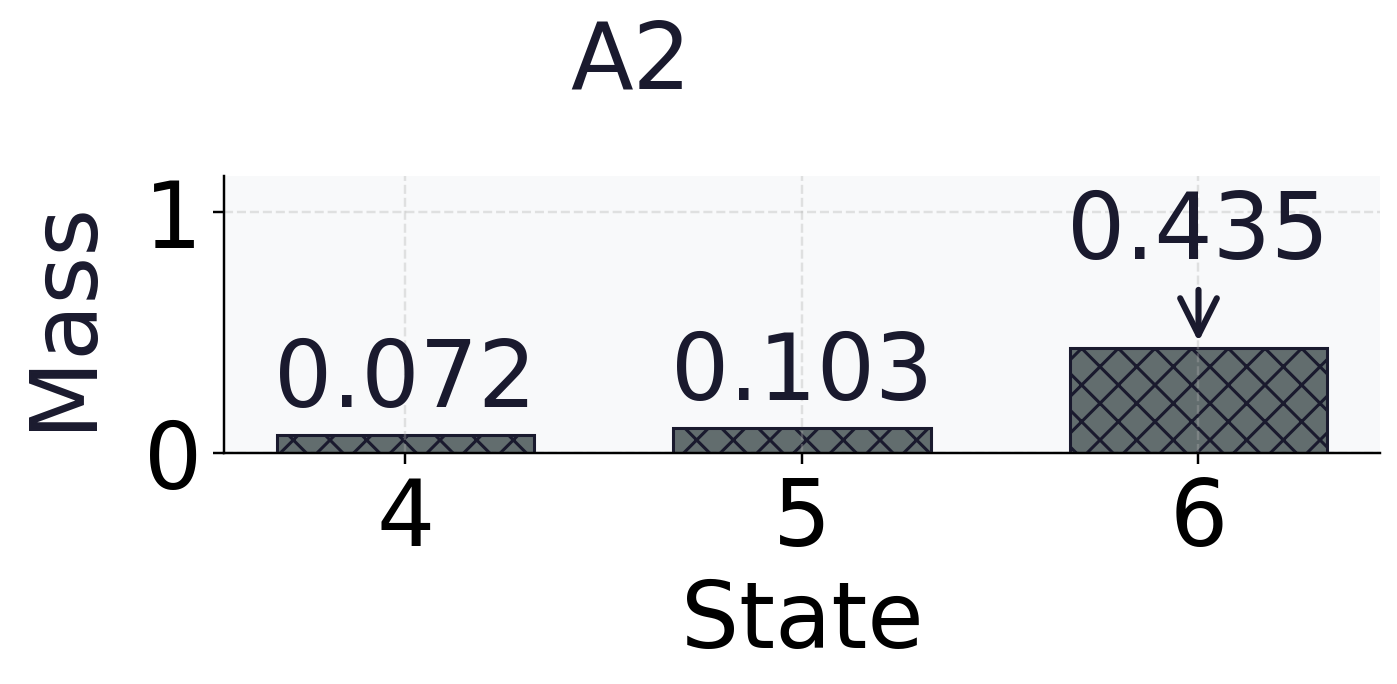
\includegraphics[keepaspectratio,width=0.98\linewidth,height=0.8\textheight,alt={A2: source-derived posterior masses for states 4 to 6, common 0--1 probability scale; arrow marks this row\textquotesingle s argmax when present.}]{../figures/system_overview.slide-row-2-states-4-6.png}
\refstepcounter{figure}\label{fig:system-overview-slide-panel-5}
\end{figure}
\end{frame}

\begin{frame}{How to read the visual\ldots{} (part 12)}
\begin{figure}
\centering
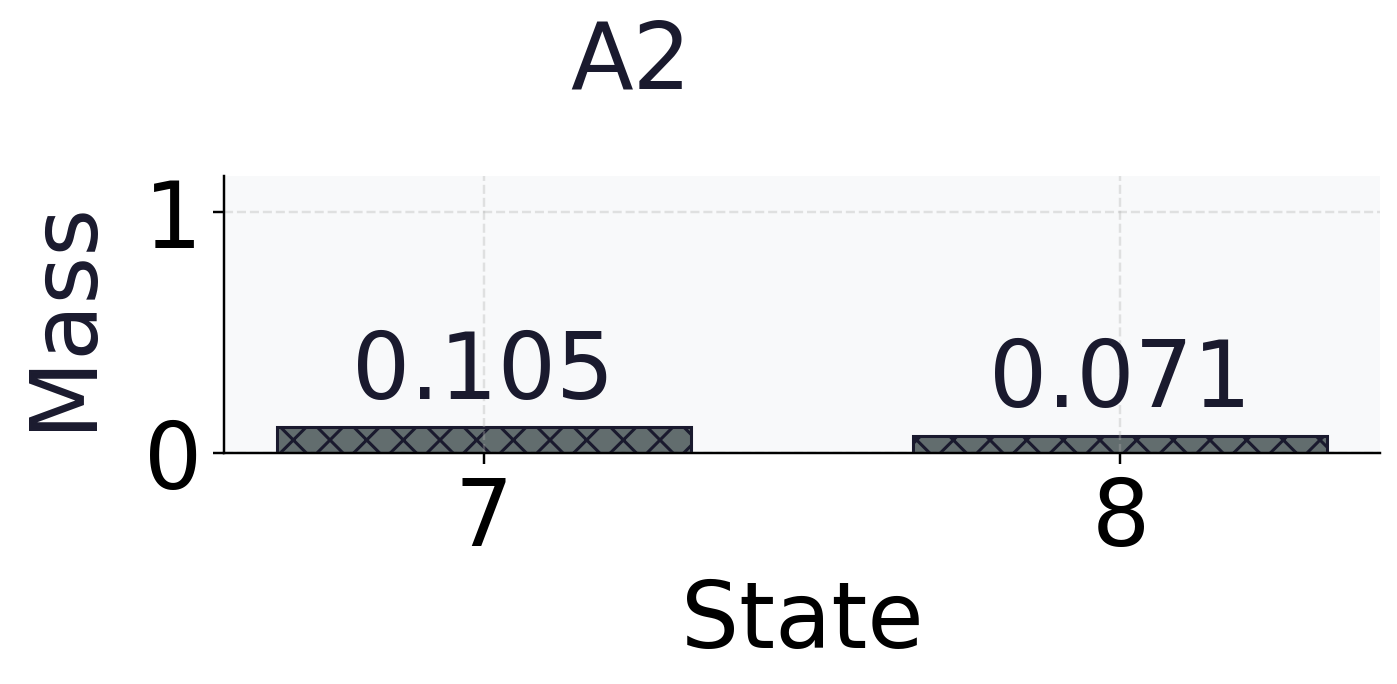
\includegraphics[keepaspectratio,width=0.98\linewidth,height=0.8\textheight,alt={A2: source-derived posterior masses for states 7 to 8, common 0--1 probability scale; arrow marks this row\textquotesingle s argmax when present.}]{../figures/system_overview.slide-row-2-states-7-8.png}
\refstepcounter{figure}\label{fig:system-overview-slide-panel-6}
\end{figure}
\end{frame}

\begin{frame}{How to read the visual\ldots{} (part 13)}
\begin{figure}
\centering
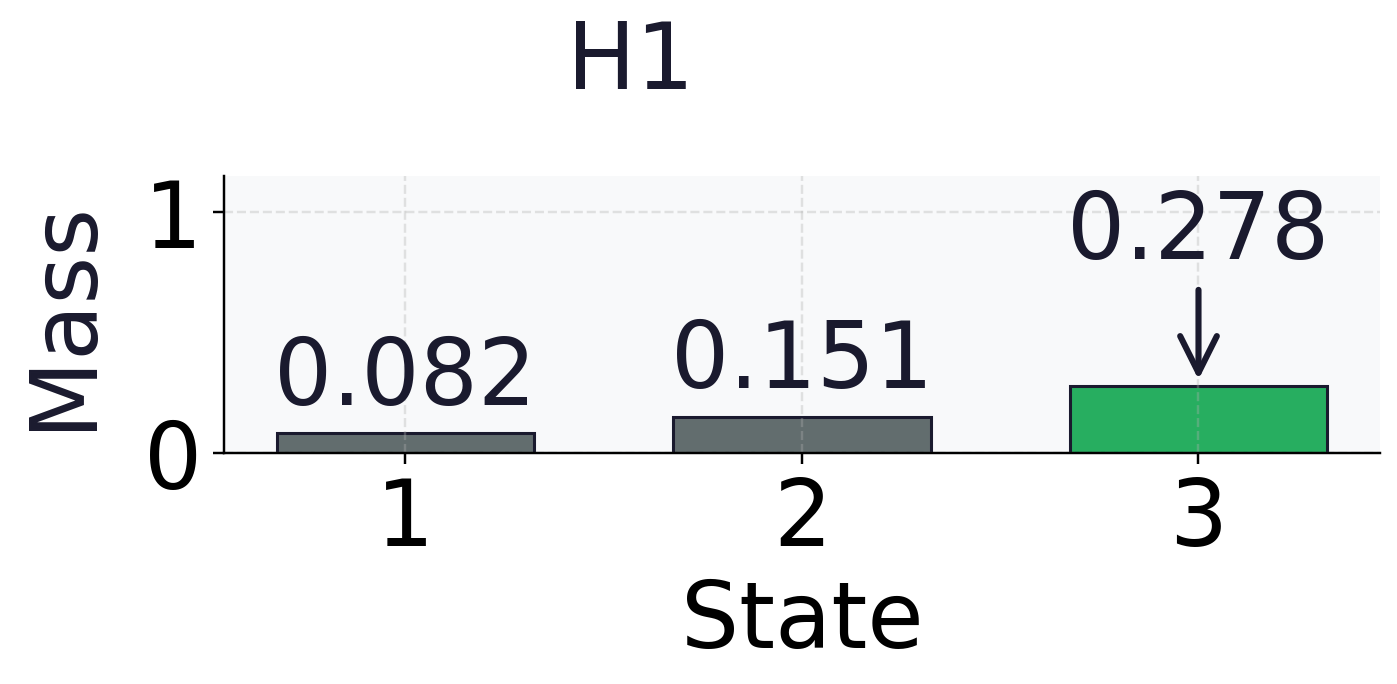
\includegraphics[keepaspectratio,width=0.98\linewidth,height=0.8\textheight,alt={H1: source-derived posterior masses for states 1 to 3, common 0--1 probability scale; arrow marks this row\textquotesingle s argmax when present.}]{../figures/system_overview.slide-row-3-states-1-3.png}
\refstepcounter{figure}\label{fig:system-overview-slide-panel-7}
\end{figure}
\end{frame}

\begin{frame}{How to read the visual\ldots{} (part 14)}
\begin{figure}
\centering
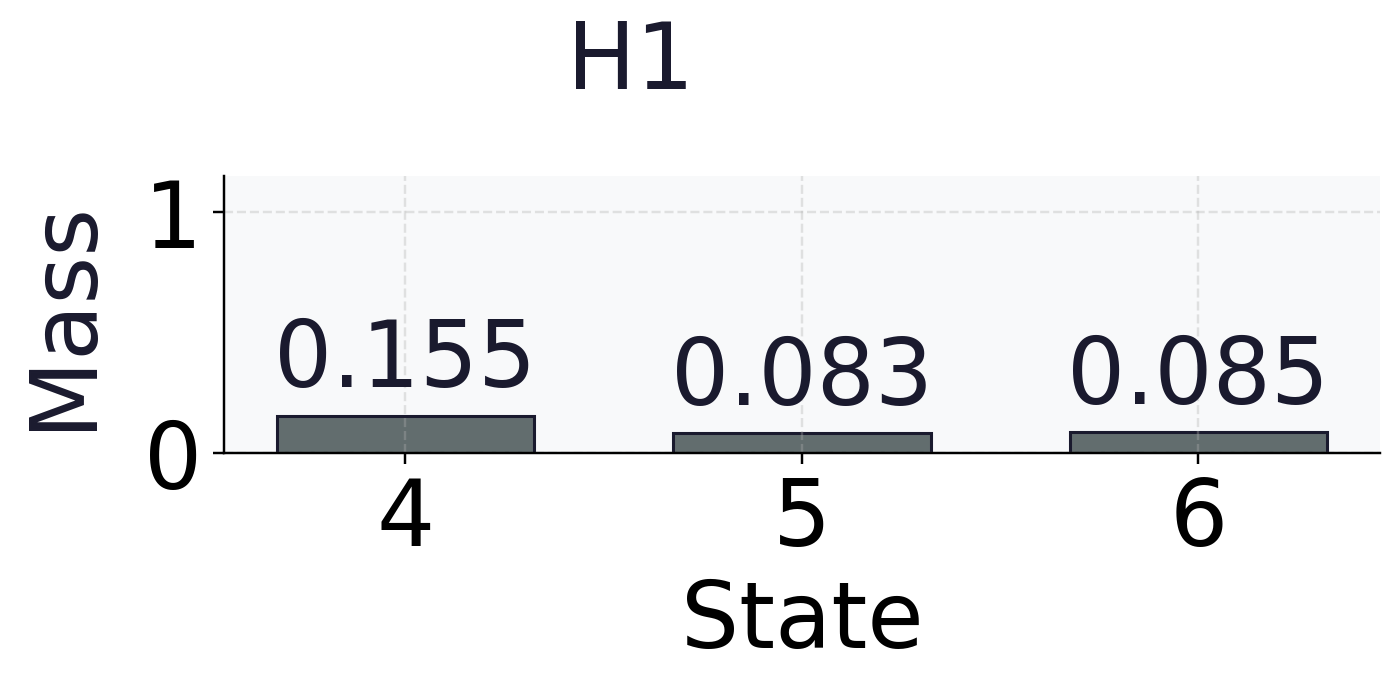
\includegraphics[keepaspectratio,width=0.98\linewidth,height=0.8\textheight,alt={H1: source-derived posterior masses for states 4 to 6, common 0--1 probability scale; arrow marks this row\textquotesingle s argmax when present.}]{../figures/system_overview.slide-row-3-states-4-6.png}
\refstepcounter{figure}\label{fig:system-overview-slide-panel-8}
\end{figure}
\end{frame}

\begin{frame}{How to read the visual\ldots{} (part 15)}
\begin{figure}
\centering
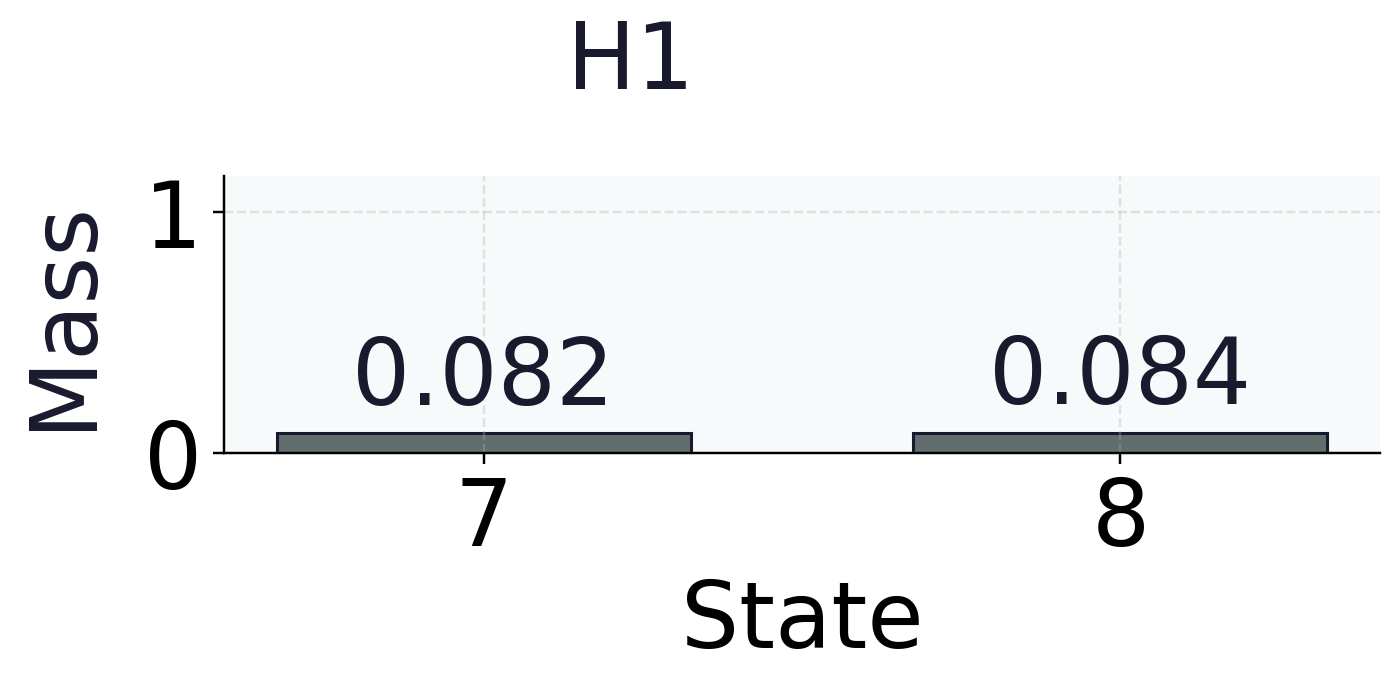
\includegraphics[keepaspectratio,width=0.98\linewidth,height=0.8\textheight,alt={H1: source-derived posterior masses for states 7 to 8, common 0--1 probability scale; arrow marks this row\textquotesingle s argmax when present.}]{../figures/system_overview.slide-row-3-states-7-8.png}
\refstepcounter{figure}\label{fig:system-overview-slide-panel-9}
\end{figure}
\end{frame}

\begin{frame}{How to read the visual\ldots{} (part 16)}
\begin{figure}
\centering
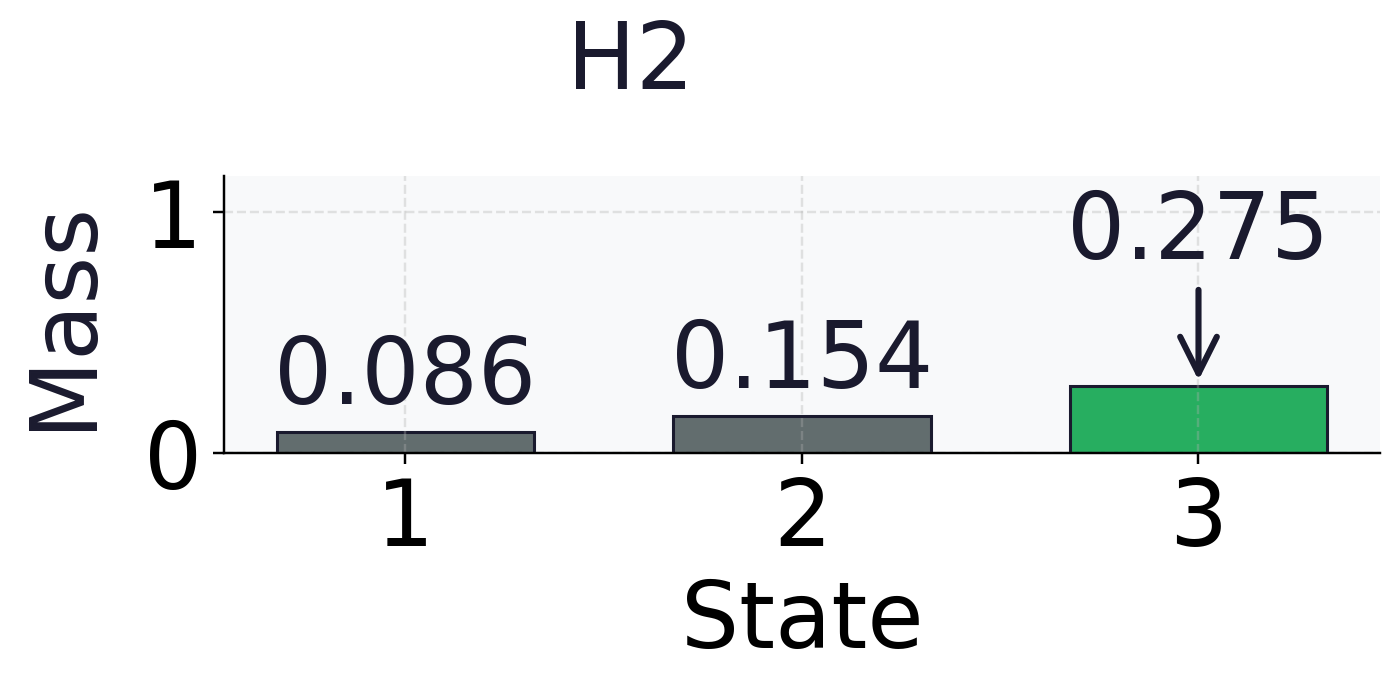
\includegraphics[keepaspectratio,width=0.98\linewidth,height=0.8\textheight,alt={H2: source-derived posterior masses for states 1 to 3, common 0--1 probability scale; arrow marks this row\textquotesingle s argmax when present.}]{../figures/system_overview.slide-row-4-states-1-3.png}
\refstepcounter{figure}\label{fig:system-overview-slide-panel-10}
\end{figure}
\end{frame}

\begin{frame}{How to read the visual\ldots{} (part 17)}
\begin{figure}
\centering
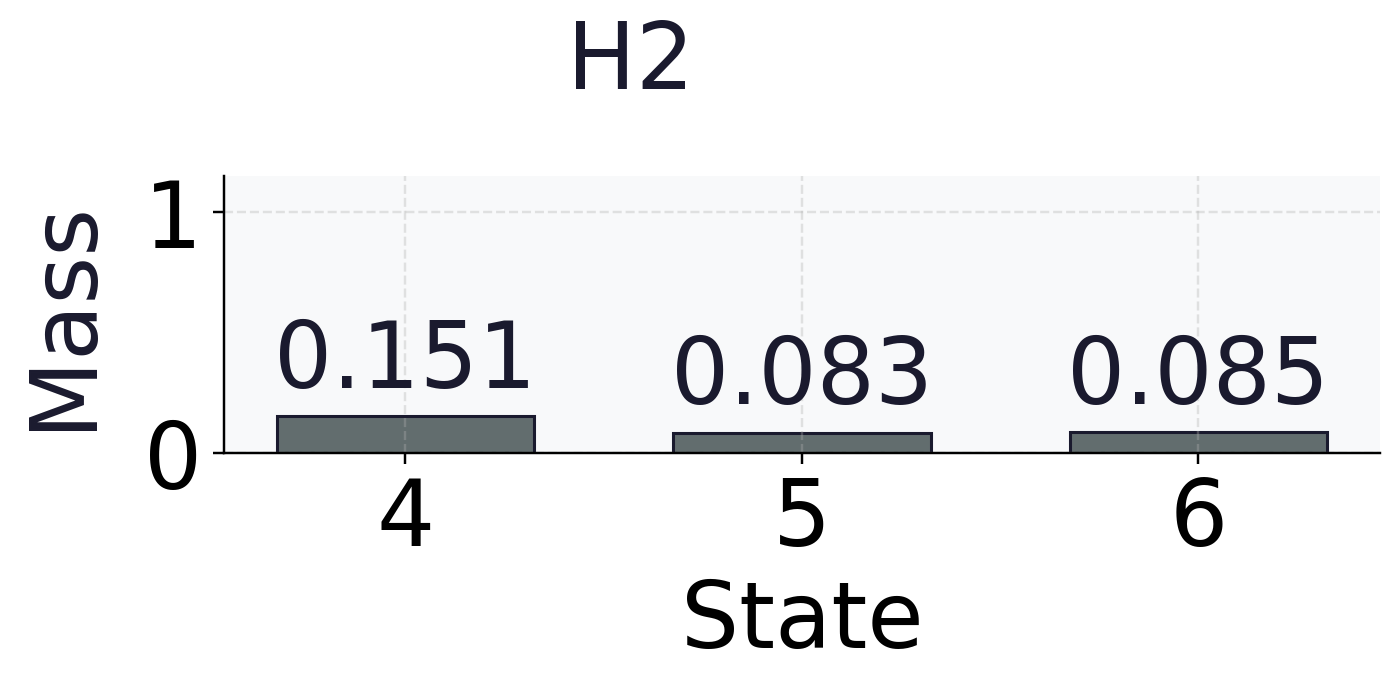
\includegraphics[keepaspectratio,width=0.98\linewidth,height=0.8\textheight,alt={H2: source-derived posterior masses for states 4 to 6, common 0--1 probability scale; arrow marks this row\textquotesingle s argmax when present.}]{../figures/system_overview.slide-row-4-states-4-6.png}
\refstepcounter{figure}\label{fig:system-overview-slide-panel-11}
\end{figure}
\end{frame}

\begin{frame}{How to read the visual\ldots{} (part 18)}
\begin{figure}
\centering
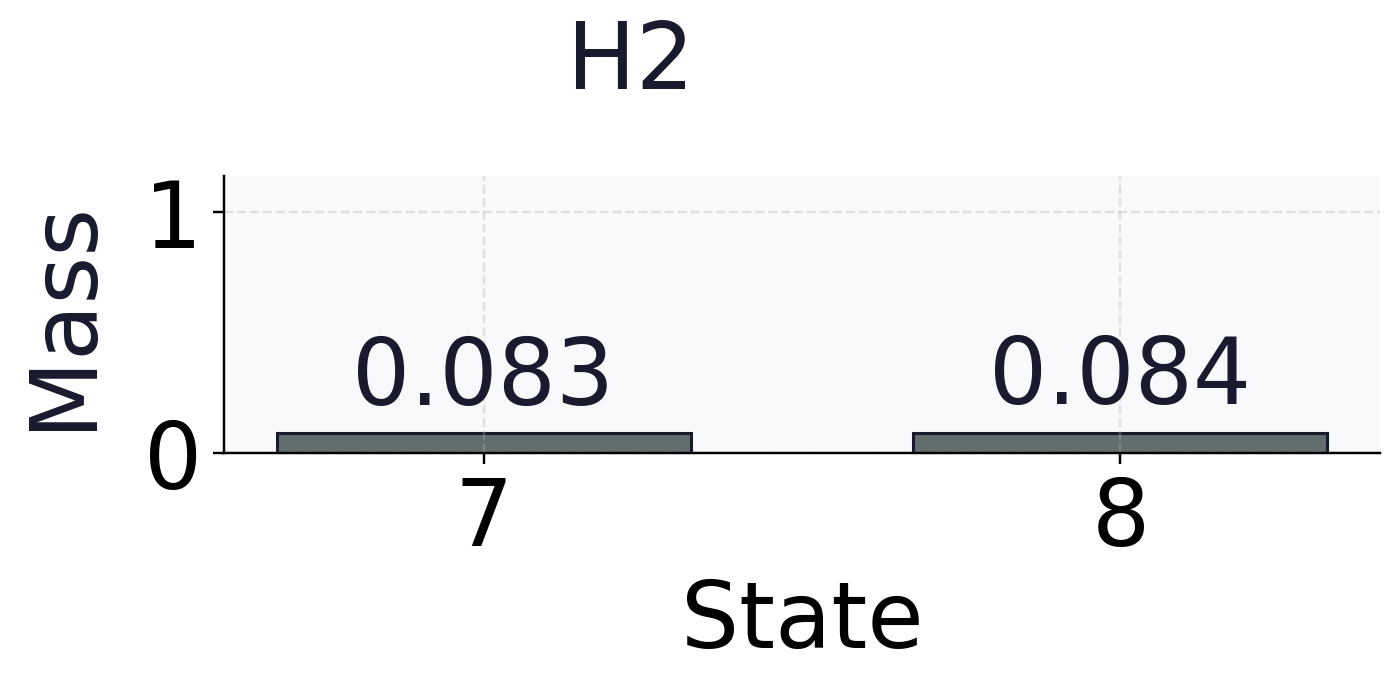
\includegraphics[keepaspectratio,width=0.98\linewidth,height=0.8\textheight,alt={H2: source-derived posterior masses for states 7 to 8, common 0--1 probability scale; arrow marks this row\textquotesingle s argmax when present.}]{../figures/system_overview.slide-row-4-states-7-8.png}
\refstepcounter{figure}\label{fig:system-overview-slide-panel-12}
\end{figure}
\end{frame}

\begin{frame}{How to read the visual\ldots{} (part 19)}
\begin{figure}
\centering
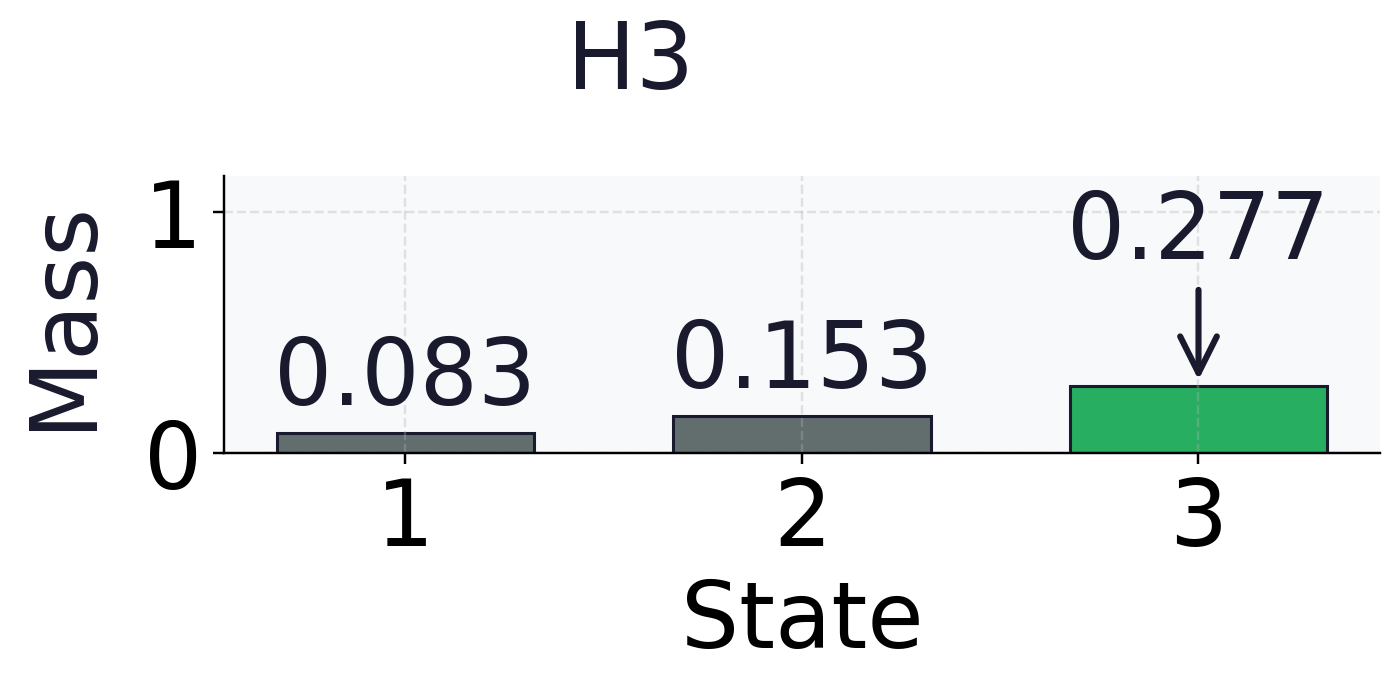
\includegraphics[keepaspectratio,width=0.98\linewidth,height=0.8\textheight,alt={H3: source-derived posterior masses for states 1 to 3, common 0--1 probability scale; arrow marks this row\textquotesingle s argmax when present.}]{../figures/system_overview.slide-row-5-states-1-3.png}
\refstepcounter{figure}\label{fig:system-overview-slide-panel-13}
\end{figure}
\end{frame}

\begin{frame}{How to read the visual\ldots{} (part 20)}
\begin{figure}
\centering
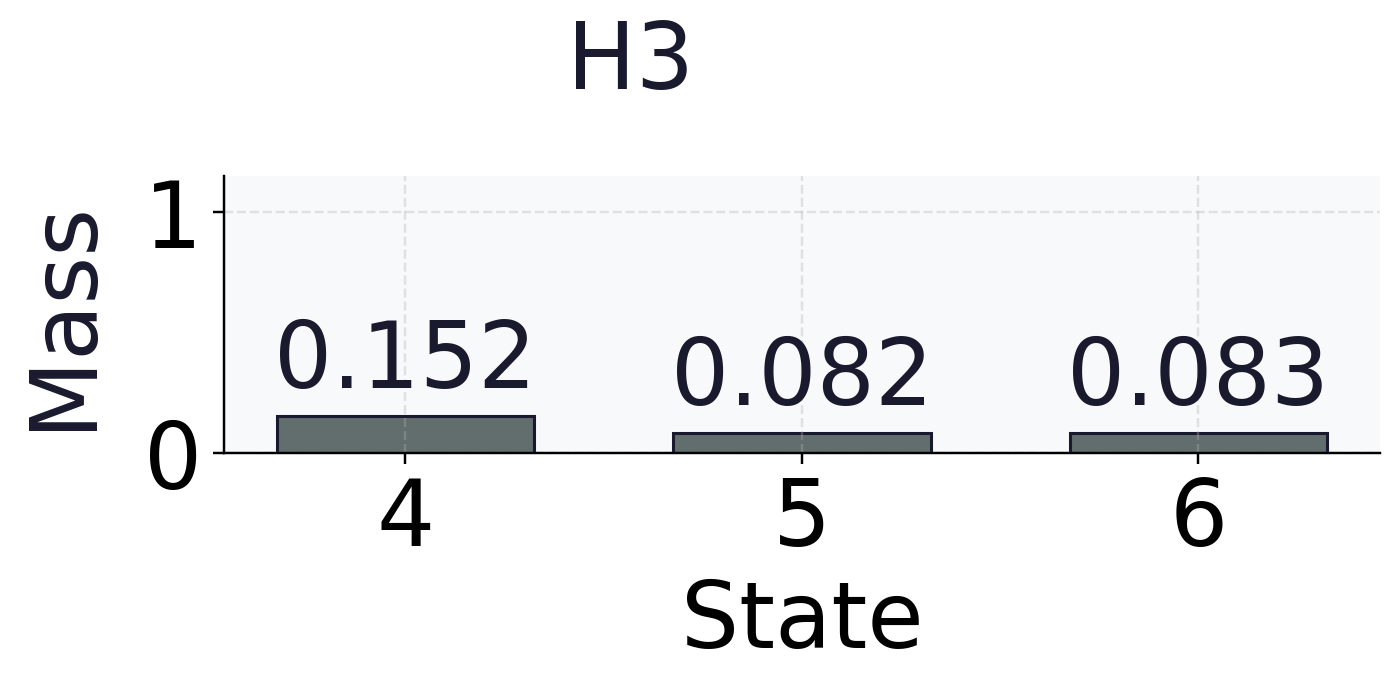
\includegraphics[keepaspectratio,width=0.98\linewidth,height=0.8\textheight,alt={H3: source-derived posterior masses for states 4 to 6, common 0--1 probability scale; arrow marks this row\textquotesingle s argmax when present.}]{../figures/system_overview.slide-row-5-states-4-6.png}
\refstepcounter{figure}\label{fig:system-overview-slide-panel-14}
\end{figure}
\end{frame}

\begin{frame}{How to read the visual\ldots{} (part 21)}
\begin{figure}
\centering
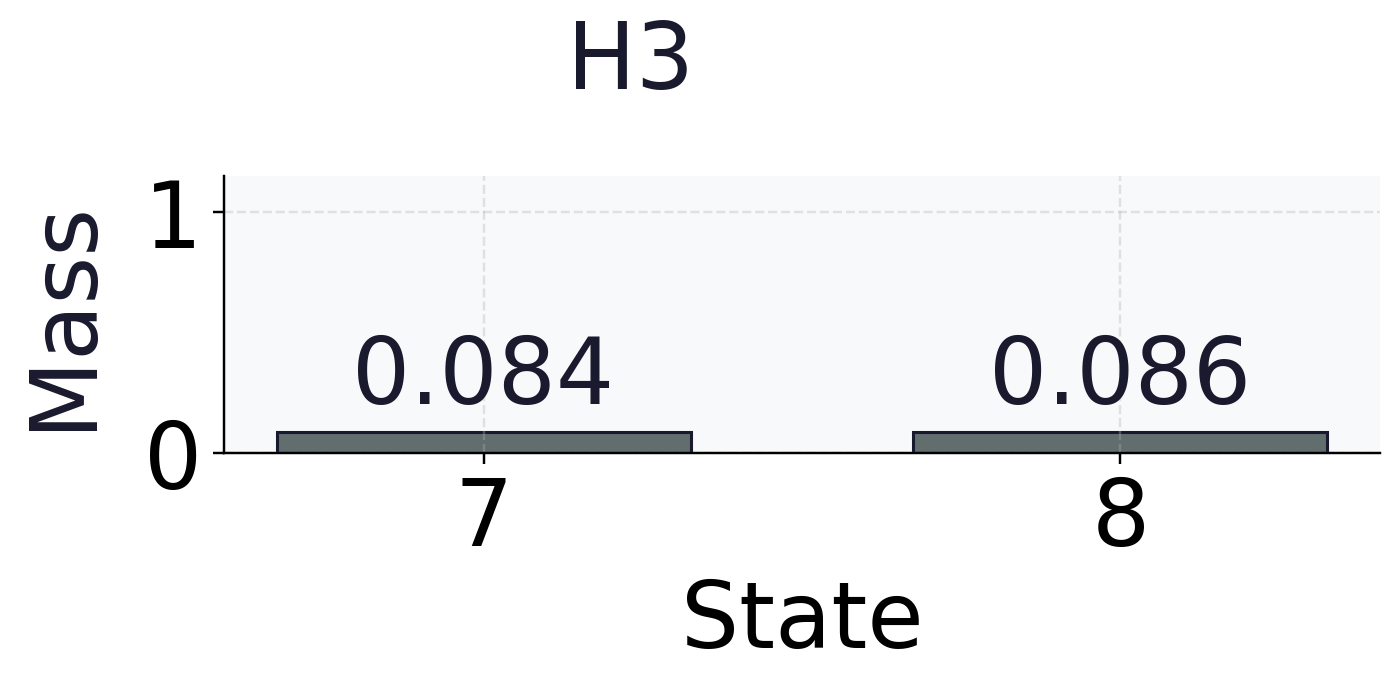
\includegraphics[keepaspectratio,width=0.98\linewidth,height=0.8\textheight,alt={H3: source-derived posterior masses for states 7 to 8, common 0--1 probability scale; arrow marks this row\textquotesingle s argmax when present.}]{../figures/system_overview.slide-row-5-states-7-8.png}
\refstepcounter{figure}\label{fig:system-overview-slide-panel-15}
\end{figure}
\end{frame}

\begin{frame}{How to read the visual\ldots{} (part 22)}
\begin{figure}
\centering
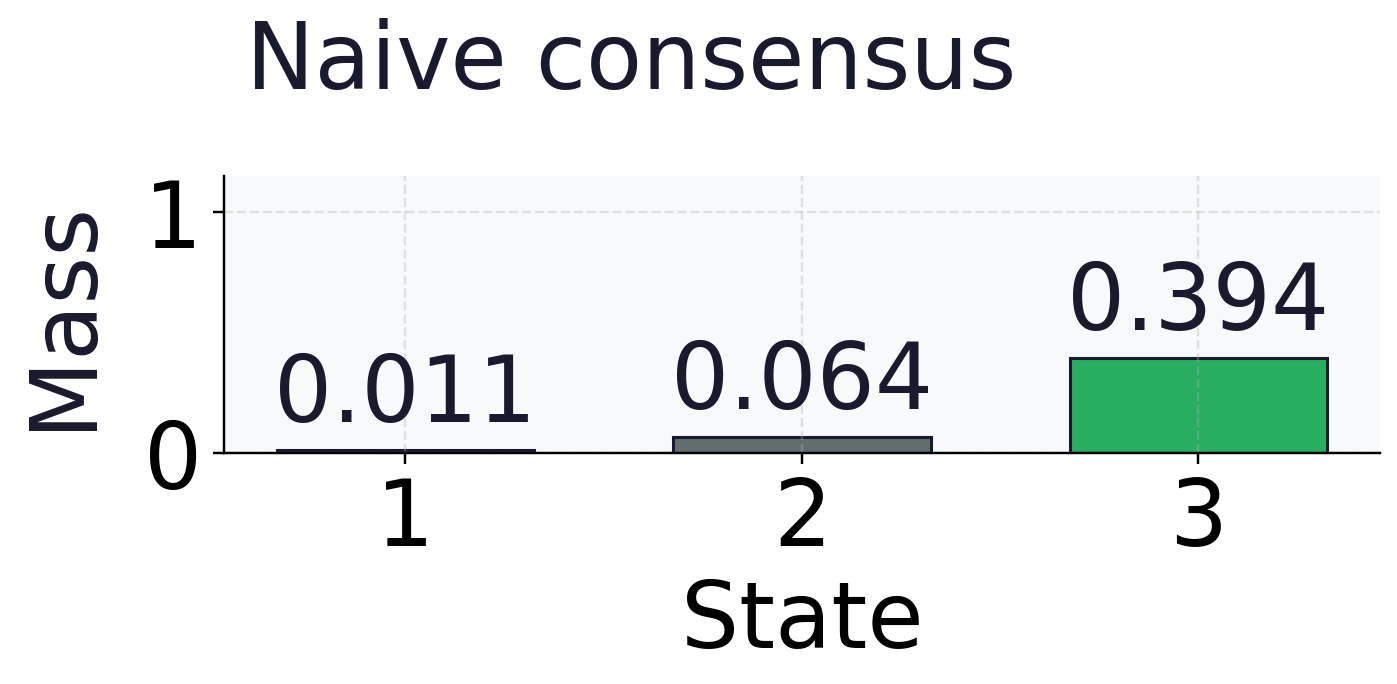
\includegraphics[keepaspectratio,width=0.98\linewidth,height=0.8\textheight,alt={Naive consensus: source-derived posterior masses for states 1 to 3, common 0--1 probability scale; arrow marks this row\textquotesingle s argmax when present.}]{../figures/system_overview.slide-row-6-states-1-3.png}
\refstepcounter{figure}\label{fig:system-overview-slide-panel-16}
\end{figure}
\end{frame}

\begin{frame}{How to read the visual\ldots{} (part 23)}
\begin{figure}
\centering
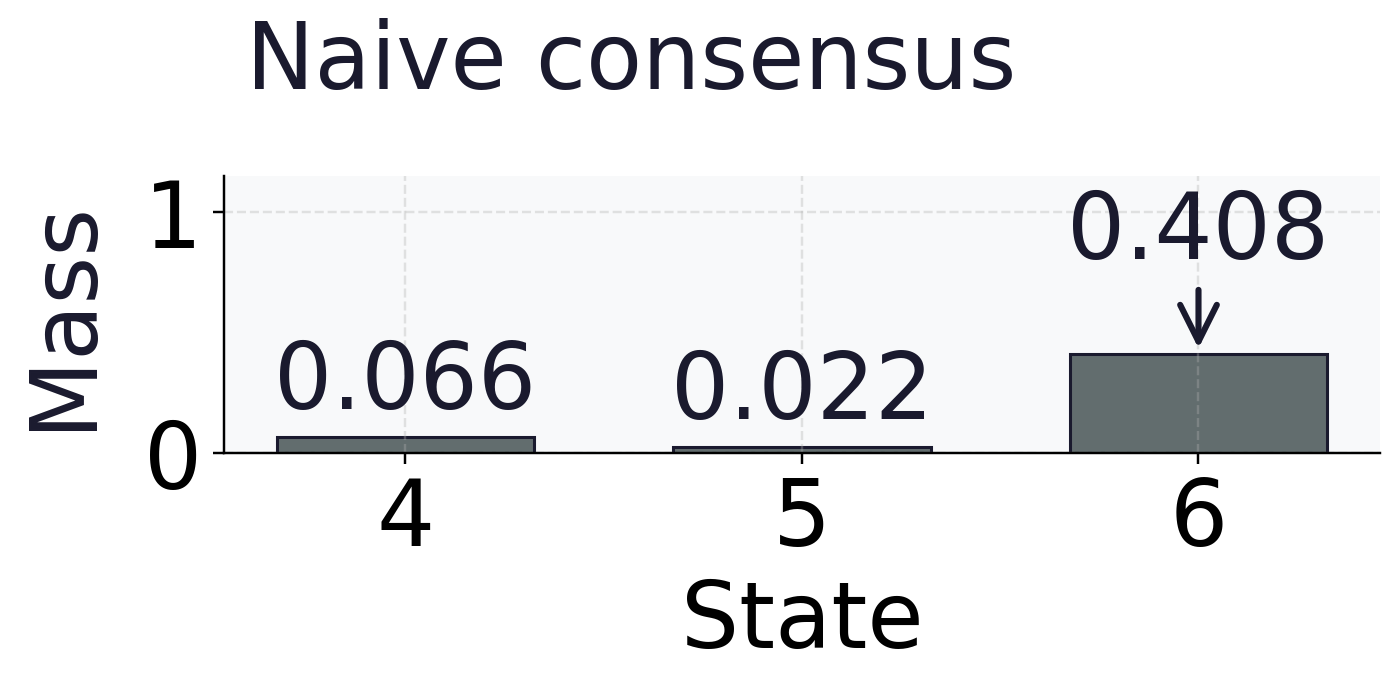
\includegraphics[keepaspectratio,width=0.98\linewidth,height=0.8\textheight,alt={Naive consensus: source-derived posterior masses for states 4 to 6, common 0--1 probability scale; arrow marks this row\textquotesingle s argmax when present.}]{../figures/system_overview.slide-row-6-states-4-6.png}
\refstepcounter{figure}\label{fig:system-overview-slide-panel-17}
\end{figure}
\end{frame}

\begin{frame}{How to read the visual\ldots{} (part 24)}
\begin{figure}
\centering
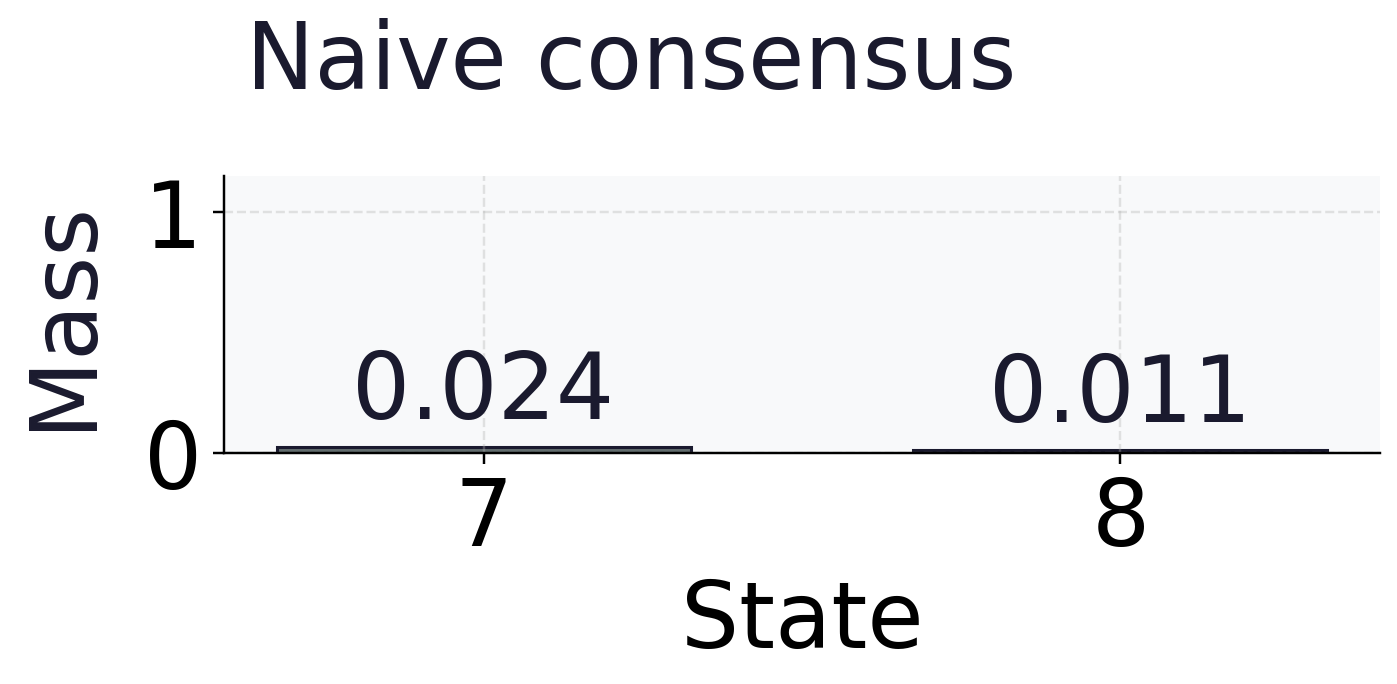
\includegraphics[keepaspectratio,width=0.98\linewidth,height=0.8\textheight,alt={Naive consensus: source-derived posterior masses for states 7 to 8, common 0--1 probability scale; arrow marks this row\textquotesingle s argmax when present.}]{../figures/system_overview.slide-row-6-states-7-8.png}
\refstepcounter{figure}\label{fig:system-overview-slide-panel-18}
\end{figure}
\end{frame}

\begin{frame}{How to read the visual\ldots{} (part 25)}
\begin{figure}
\centering
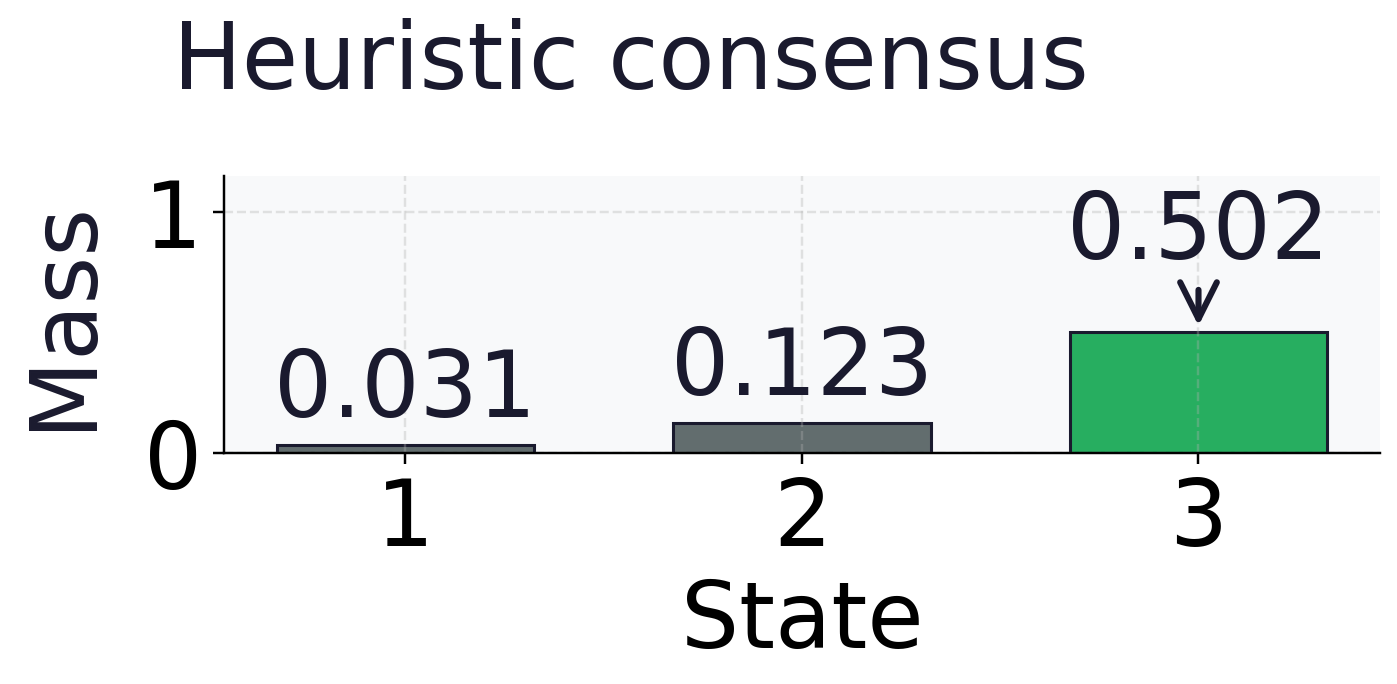
\includegraphics[keepaspectratio,width=0.98\linewidth,height=0.8\textheight,alt={Heuristic consensus: source-derived posterior masses for states 1 to 3, common 0--1 probability scale; arrow marks this row\textquotesingle s argmax when present.}]{../figures/system_overview.slide-row-7-states-1-3.png}
\refstepcounter{figure}\label{fig:system-overview-slide-panel-19}
\end{figure}
\end{frame}

\begin{frame}{How to read the visual\ldots{} (part 26)}
\begin{figure}
\centering
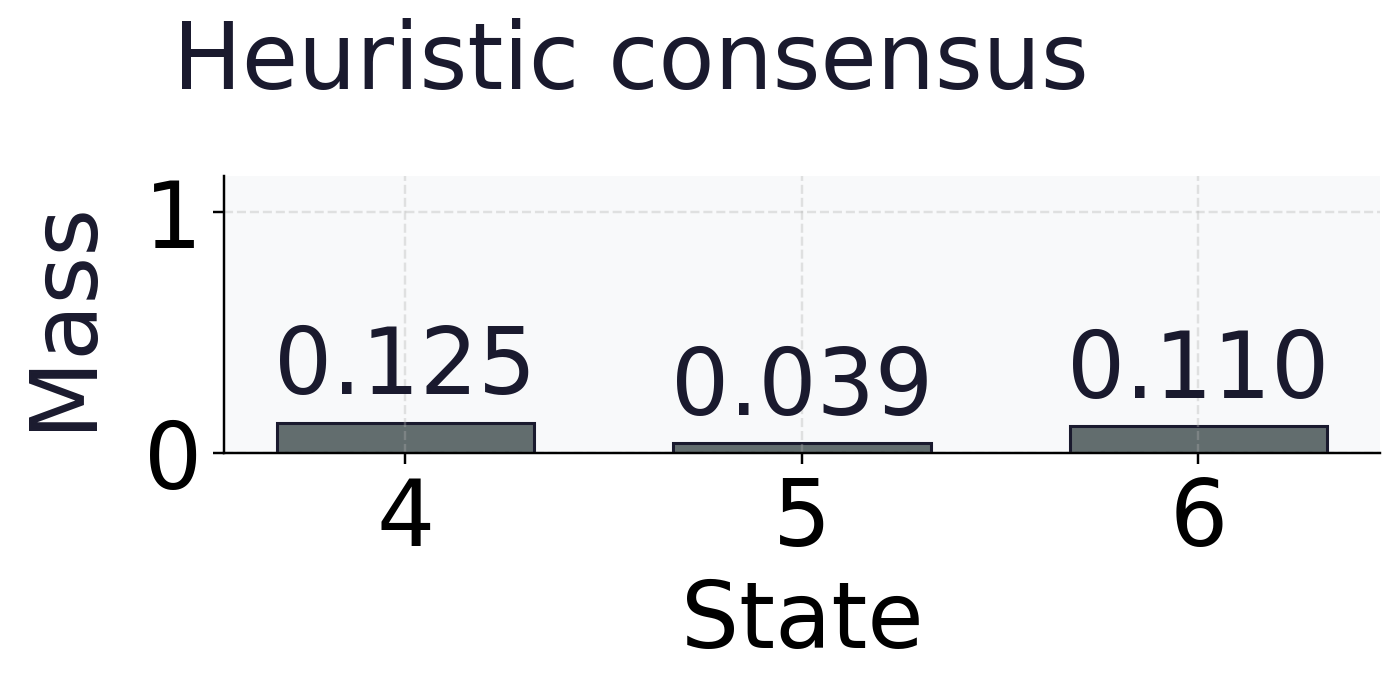
\includegraphics[keepaspectratio,width=0.98\linewidth,height=0.8\textheight,alt={Heuristic consensus: source-derived posterior masses for states 4 to 6, common 0--1 probability scale; arrow marks this row\textquotesingle s argmax when present.}]{../figures/system_overview.slide-row-7-states-4-6.png}
\refstepcounter{figure}\label{fig:system-overview-slide-panel-20}
\end{figure}
\end{frame}

\begin{frame}{How to read the visual\ldots{} (part 27)}
\begin{figure}
\centering
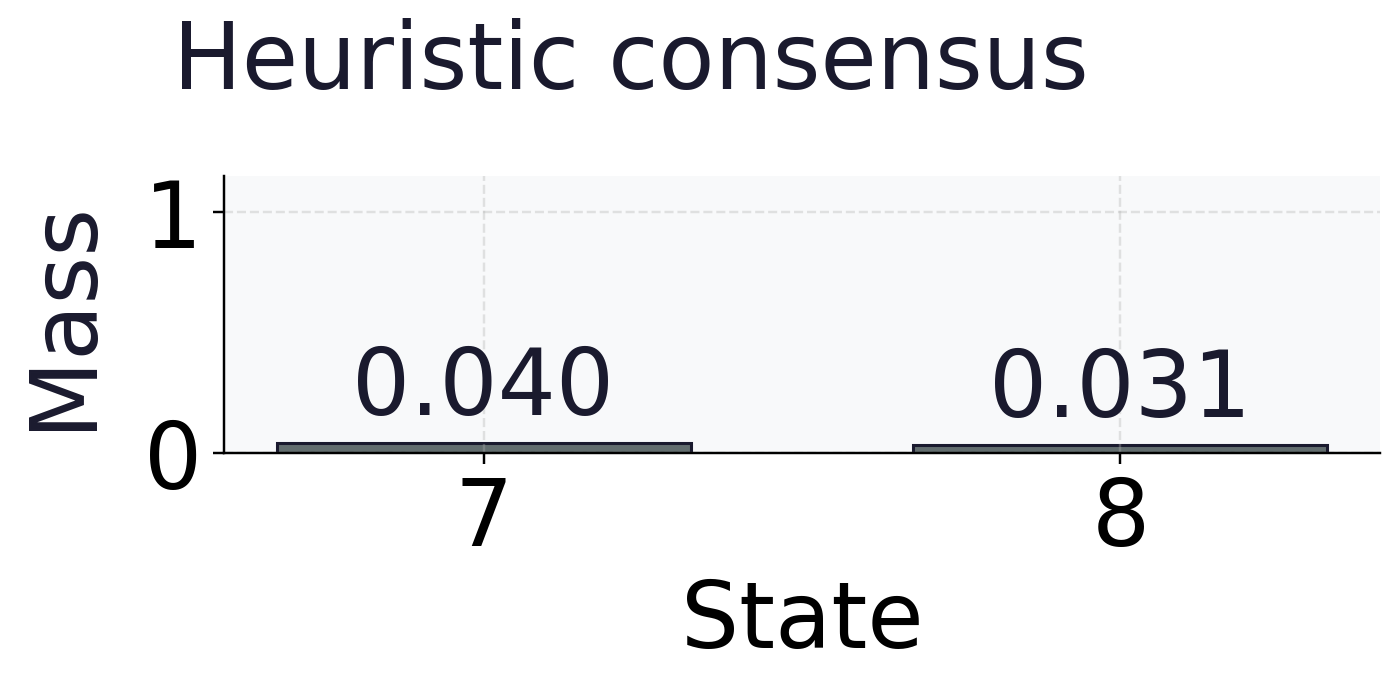
\includegraphics[keepaspectratio,width=0.98\linewidth,height=0.8\textheight,alt={Heuristic consensus: source-derived posterior masses for states 7 to 8, common 0--1 probability scale; arrow marks this row\textquotesingle s argmax when present.}]{../figures/system_overview.slide-row-7-states-7-8.png}
\refstepcounter{figure}\label{fig:system-overview-slide-panel-21}
\end{figure}
\end{frame}

\begin{frame}{How to read the visual\ldots{} (part 28)}
\begin{figure}
\centering
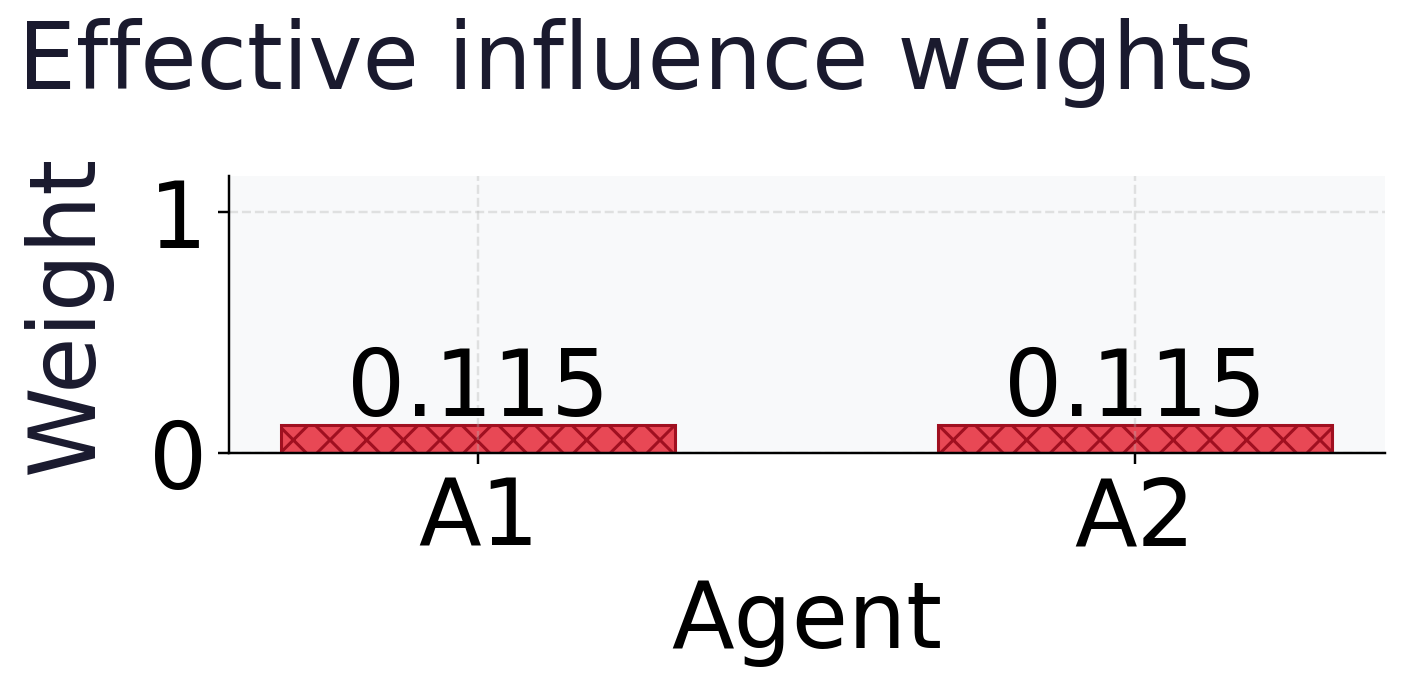
\includegraphics[keepaspectratio,width=0.98\linewidth,height=0.8\textheight,alt={Source-derived normalized heuristic influence weights; adversarial bars are crosshatched and agent labels preserve their roles.}]{../figures/system_overview.slide-weights-1-2.png}
\refstepcounter{figure}\label{fig:system-overview-slide-panel-22}
\end{figure}
\end{frame}

\begin{frame}{How to read the visual\ldots{} (part 29)}
\begin{figure}
\centering
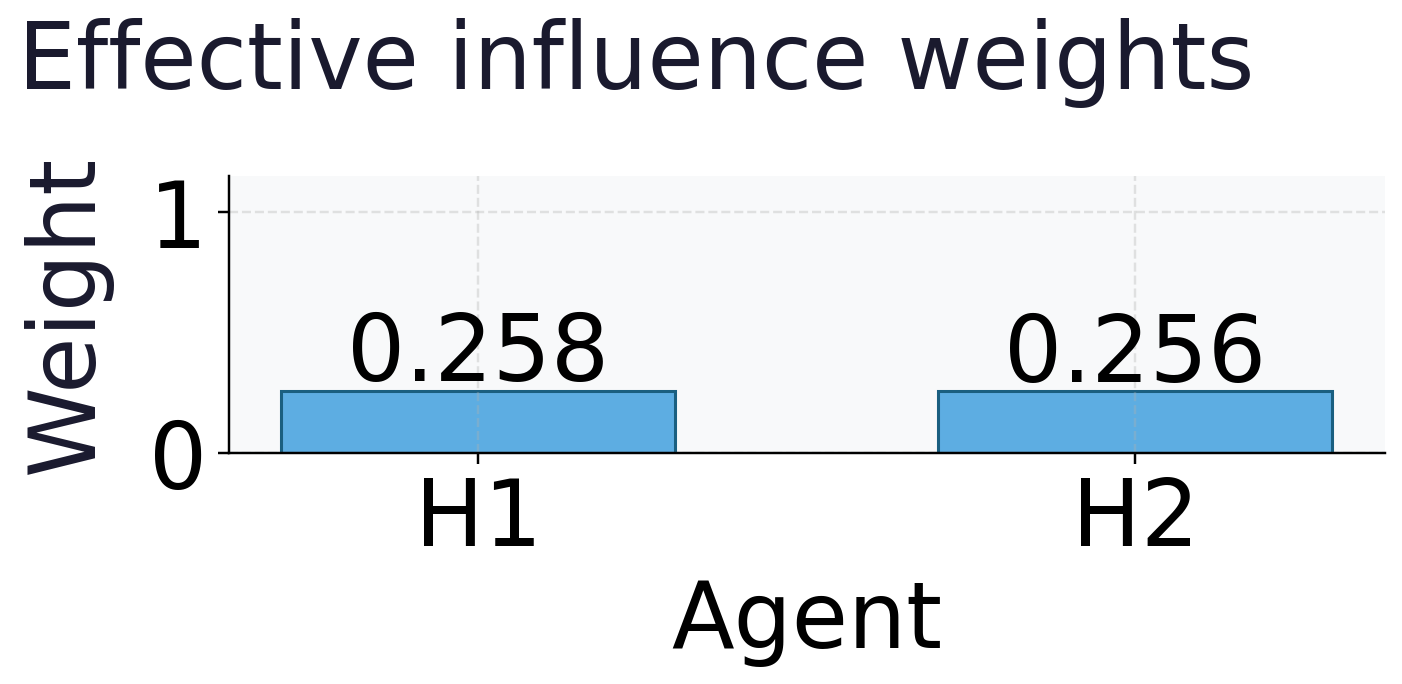
\includegraphics[keepaspectratio,width=0.98\linewidth,height=0.8\textheight,alt={Source-derived normalized heuristic influence weights; adversarial bars are crosshatched and agent labels preserve their roles.}]{../figures/system_overview.slide-weights-3-4.png}
\refstepcounter{figure}\label{fig:system-overview-slide-panel-23}
\end{figure}
\end{frame}

\begin{frame}{How to read the visual\ldots{} (part 30)}
\begin{figure}
\centering
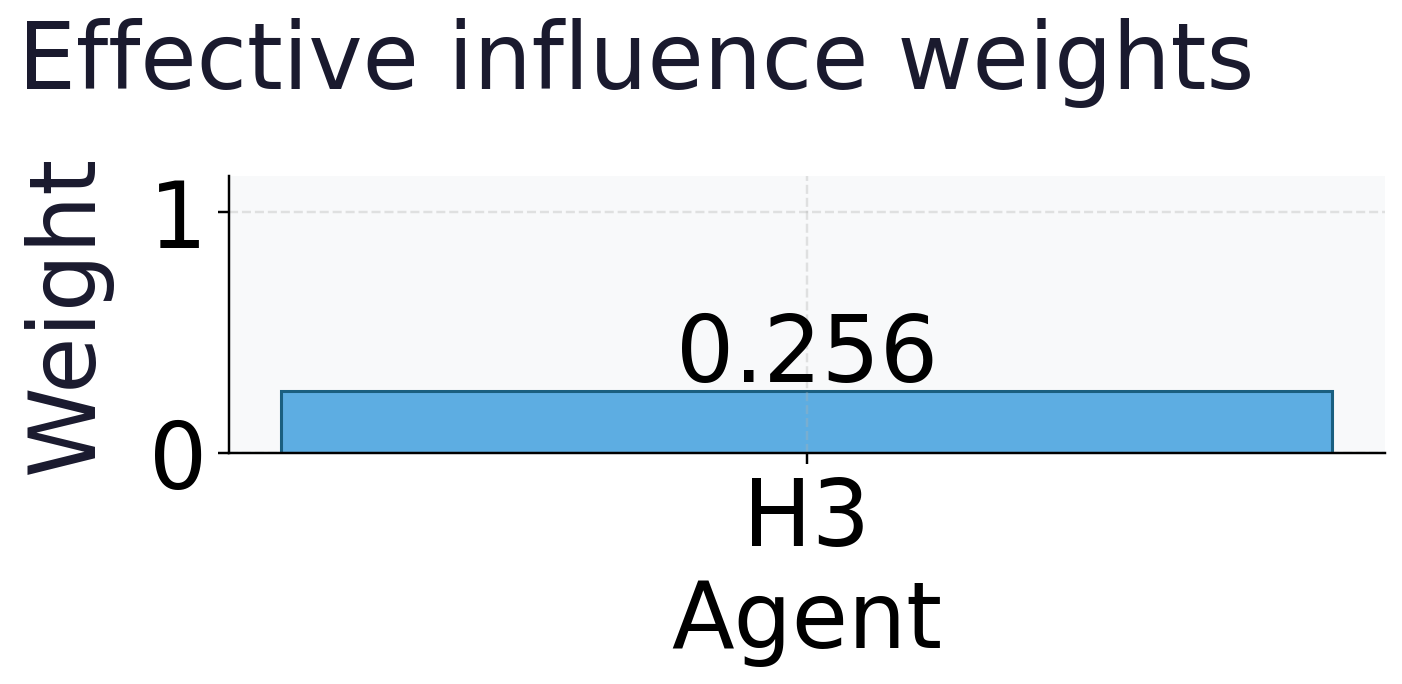
\includegraphics[keepaspectratio,width=0.98\linewidth,height=0.8\textheight,alt={Source-derived normalized heuristic influence weights; adversarial bars are crosshatched and agent labels preserve their roles.}]{../figures/system_overview.slide-weights-5-5.png}
\refstepcounter{figure}\label{fig:system-overview-slide-panel-24}
\end{figure}
\end{frame}

\begin{frame}{How to read the visual\ldots{} (part 31)}
\begin{figure}
\centering
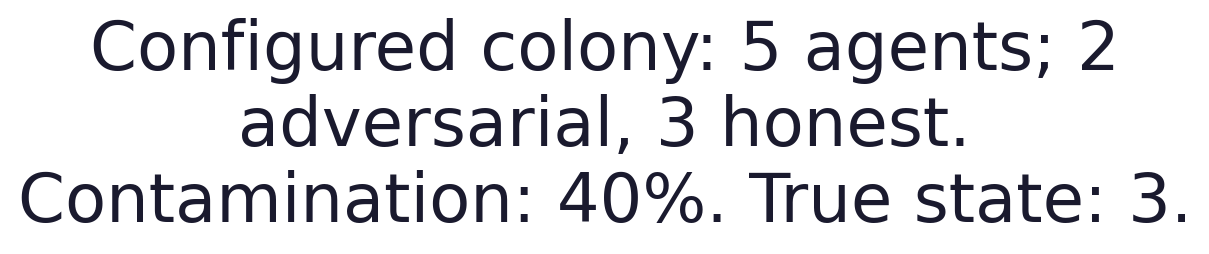
\includegraphics[keepaspectratio,width=0.98\linewidth,height=0.8\textheight,alt={Configured colony: 5 agents; 2 adversarial, 3 honest. Contamination: 40\%. True state: 3.}]{../figures/system_overview.slide-colony.png}
\refstepcounter{figure}\label{fig:system-overview-slide-panel-25}
\end{figure}
\end{frame}

\begin{frame}{How to read the visual\ldots{} (part 32)}
\begin{figure}
\centering

\includegraphics[keepaspectratio,width=0.98\linewidth,height=0.8\textheight,alt={Naive equal-weight log pool: true-state mass 39\%; argmax state 6.}]{../figures/system_overview.slide-naive.png}
\refstepcounter{figure}\label{fig:system-overview-slide-panel-26}
\end{figure}
\end{frame}

\begin{frame}{How to read the visual\ldots{} (part 33)}
\begin{figure}
\centering
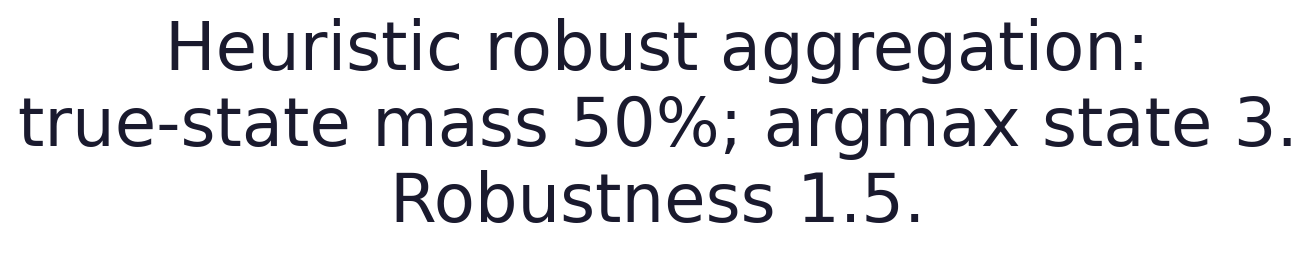
\includegraphics[keepaspectratio,width=0.98\linewidth,height=0.8\textheight,alt={Heuristic robust aggregation: true-state mass 50\%; argmax state 3. Robustness 1.5.}]{../figures/system_overview.slide-heuristic.png}
\refstepcounter{figure}\label{fig:system-overview-slide-panel-27}
\end{figure}
\end{frame}

\begin{frame}{How to read the visual\ldots{} (part 34)}
\begin{figure}
\centering
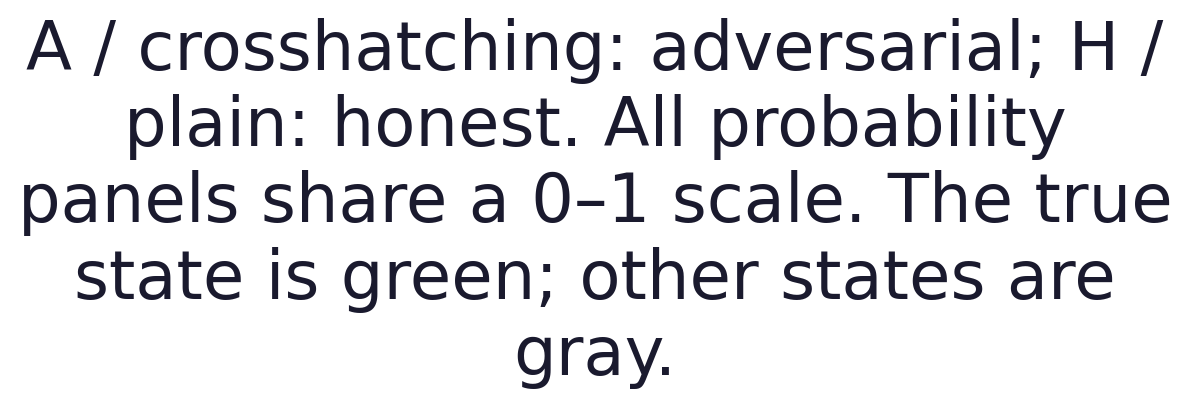
\includegraphics[keepaspectratio,width=0.98\linewidth,height=0.8\textheight,alt={A / crosshatching: adversarial; H / plain: honest. All probability panels share a 0--1 scale. The true state is green; other states are gray.}]{../figures/system_overview.slide-key.png}
\refstepcounter{figure}\label{fig:system-overview-slide-panel-28}
\end{figure}
\end{frame}

\begin{frame}{How to read the visual\ldots{} (part 35)}
\begin{figure}
\centering
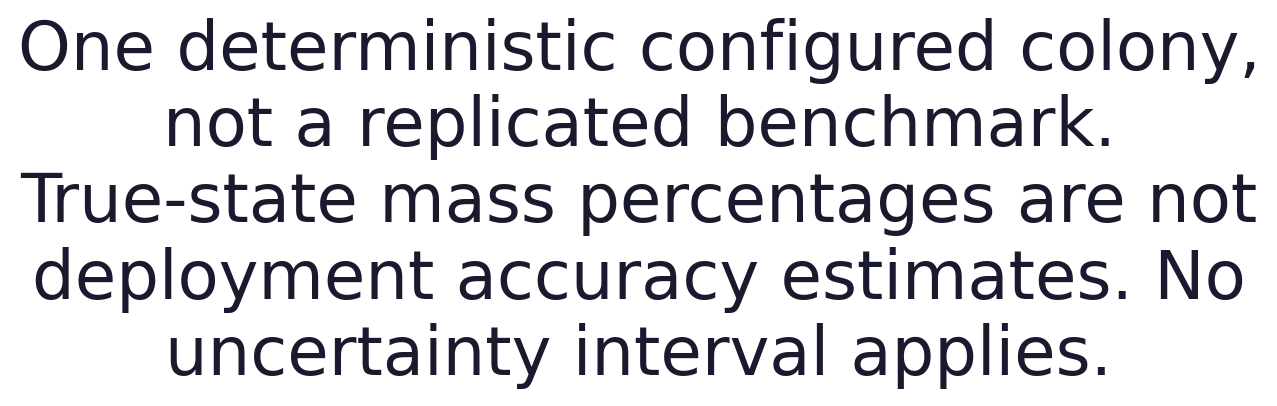
\includegraphics[keepaspectratio,width=0.98\linewidth,height=0.8\textheight,alt={One deterministic configured colony, not a replicated benchmark. True-state mass percentages are not deployment accuracy estimates. No uncertainty interval applies.}]{../figures/system_overview.slide-scope.png}
\refstepcounter{figure}\label{fig:system-overview-slide-panel-29}
\end{figure}
\end{frame}

\end{document}
